%-----------------------------------------------------------------------------
%
%               Template for sigplanconf LaTeX Class
%
% Name:         sigplanconf-template.tex
%
% Purpose:      A template for sigplanconf.cls, which is a LaTeX 2e class
%               file for SIGPLAN conference proceedings.
%
% Guide:        Refer to "Author's Guide to the ACM SIGPLAN Class,"
%               sigplanconf-guide.pdf
%
% Author:       Paul C. Anagnostopoulos
%               Windfall Software
%               978 371-2316
%               paul@windfall.com
%
% Created:      15 February 2005
%
%-----------------------------------------------------------------------------


%\documentclass[preprint,numbers]{sigplanconf}
\documentclass[acmlarge,anonymous]{acmart}\settopmatter{printfolios=true}

% The following \documentclass options may be useful:

% preprint      Remove this option only once the paper is in final form.
% 10pt          To set in 10-point type instead of 9-point.
% 11pt          To set in 11-point type instead of 9-point.
% numbers       To obtain numeric citation style instead of author/year.

\usepackage{amssymb}
\usepackage{amsmath}
\usepackage{amsfonts}
\usepackage{caption}
\usepackage{subcaption}
\usepackage{xspace}
\usepackage{mathtools}
\usepackage{mathpartir}
\usepackage{ifpdf}
\usepackage{graphicx}
%\usepackage[usenames,dvipsnames]{color}
\usepackage{stmaryrd}
%\usepackage[numbers]{natbib}
\usepackage{amsthm}
\usepackage{listings}          % format code
\usepackage{wrapfig}
\usepackage{textcomp}
\usepackage{tabularx}
\usepackage{color}
\usepackage{url}
\usepackage{tikz}


% Math mode
%-----------
\newenvironment{nop}{}{}
\newenvironment{smathpar}{
\begin{nop}\small\begin{mathpar}}{
\end{mathpar}\end{nop}\ignorespacesafterend}

% Theorem
%--------

% \theoremstyle{plain}
% \newtheorem{axiom}{Axiom}[section]
% \newtheorem{theorem}{Theorem}[section]
% \newtheorem{lemma}[theorem]{Lemma}
% \newtheorem{proposition}[theorem]{Proposition}
% \newtheorem{corollary}[theorem]{Corollary}
% \theoremstyle{definition}
% \newtheorem{definition}[theorem]{Definition}

% \newenvironment{example}[1][Example]{\begin{trivlist}
% \item[\hskip \labelsep {\bfseries #1}]}{\end{trivlist}}
% \newenvironment{remark}[1][Remark]{\begin{trivlist}
% \item[\hskip \labelsep {\bfseries #1}]}{\end{trivlist}}

% Decorations
%-----------
\newenvironment{decoration}
  {\color{blue}\begin{array}{l}}
  {\end{array}}

% New colors
%------------
\definecolor{Bittersweet}{rgb}{1.0, 0.44, 0.37}
\definecolor{MidnightBlue}{rgb}{0.0, 0.2, 0.4}

% Listings
%----------
\newcommand{\lsttxnimp}{\lstset{
      language=c,
      basicstyle=\ttfamily\small,
      flexiblecolumns=false,
			tabsize=2,
      escapechar=',                        
      %basewidth={0.5em,0.45em},
      %aboveskip={3pt},
      %belowskip={3pt},
      keywordstyle=\color{Bittersweet}\bfseries,
      commentstyle=\color{blue}\itshape,
      stringstyle=\color{MidnightBlue},
      morekeywords={transaction,txn,cobegin,from,to,atomic},
			classoffset=1,
			upquote=true,
			keywordstyle=\color{Fuchsia}\bfseries,
			classoffset=0,
			mathescape=true
    }}
\lstnewenvironment{txnimpcode}
    { % \centering
      \lsttxnimp
      \lstset{}%
      \csname lst@setfirstlabel\endcsname}
    { %\centering
      \csname lst@savefirstlabel\endcsname}

% Listings Code
%---------------
\newcommand{\lstml}{
\lstset{ %
language=ML, % choose the language of the code
basicstyle=\footnotesize\ttfamily,       % the size of the fonts that are used for the code
keywordstyle=\color{Bittersweet},
% numbers=left,                   % where to put the line-numbers
numberstyle=\tiny,      % the size of the fonts that are used for the line-numbers
stepnumber=1,                   % the step between two line-numbers. If it is 1 each line will be numbered
numbersep=5pt,                  % how far the line-numbers are from the code
showspaces=false,               % show spaces adding particular underscores
showstringspaces=false,         % underline spaces within strings
showtabs=false,                 % show tabs within strings adding particular underscores
% frame=single,                   % adds a frame around the code
tabsize=2,                      % sets default tabsize to 2 spaces
captionpos=b,                   % sets the caption-position to bottom
breaklines=true,                % sets automatic line breaking
breakatwhitespace=false,        % sets if automatic breaks should only happen at whitespace
commentstyle=\itshape\color{MidnightBlue},
%escapeinside={\%*}{*)},         % if you want to add a comment within your code
mathescape=true,
morekeywords={module, match, when, @@deriving, not, : , txn_do, do, SQL/\\}
}}
\lstnewenvironment{ocaml}
    { % \centering
			\lstml
      \lstset{}%
      \csname lst@setfirstlabel\endcsname}
    { %\centering
      \csname lst@savefirstlabel\endcsname}
\newcommand{\ocamlinline}[1]{\lstinline[language=ML,
                                        basicstyle=\footnotesize\ttfamily, 
                                        keywordstyle=\color{Bittersweet},
                                        mathescape=true]{#1}}

% Formatting
%---------
\newcommand{\C}[1]{\code{#1}}
%\newcommand{\R}[1]{\textsc{#1}}
\newcommand{\tuplee}[1]{\langle #1 \rangle}
\newcommand*{\rom}[1]{\expandafter\romannumeral #1}

% Formatting commands
% -------------------
\newcommand{\code}[1]{{\tt #1}}
\newcommand{\spc}[0]{\quad}
\newcommand{\ALT}{~\mid~}
\newcommand{\rel}[1]{{R}_{\mathit{#1}}}
\newcommand{\conj}{~\wedge~}
\newcommand{\disj}{~\vee~}
\newcommand{\rulelabel}[1]{\textrm{\sc {#1}}}
\newcommand{\ilrulelabel}[1]{{\sc #1}}
\newcommand{\RULE}[2]{\frac{\begin{array}{c}#1\end{array}}
                           {\begin{array}{c}#2\end{array}}}
\newcommand{\txnimp}{\mbox{${\mathcal T}$}}
%\newcommand{\coloneqq}{::=}
\newcommand{\qqquad}{\quad\quad}
\newcommand{\cskip}{\C{SKIP}}
\newcommand{\ctxnr}[3]{{\sf txn}_{#1}\langle #2 \rangle\{#3\}}
\newcommand{\ctxn}[3]{\C{TXN}_{#1}\langle #2 \rangle\{#3\}}
\newcommand{\catomic}[1]{\C{ATOMIC}\{#1\}}
\newcommand{\stepsto}{\longrightarrow}
\newcommand{\rstepsto}{\longrightarrow_{R}}
\newcommand{\stepssto}[1]{\longrightarrow^{#1}_{R}}
\newcommand{\rstepssto}[1]{\longrightarrow^{#1}_{R}}
\newcommand{\xstepsto}[1]{\longrightarrow_{#1}}
\newcommand{\xstepssto}[2]{\longrightarrow^{#1}_{#2}}
\newcommand{\tstepsto}{\longrightarrow}
\newcommand{\redsto}{\hookrightarrow}
\newcommand{\xtstepsto}[1]{\hookrightarrow_{#1}}
\newcommand{\rtstepsto}{\hookrightarrow_R}
\newcommand{\rtstepssto}[1]{\hookrightarrow^{#1}_R}
\newcommand{\xtstepssto}[2]{\hookrightarrow^{#1}_{#2}}
\newcommand{\hoare}[3]{\{#1\}\,#2\,\{#3\}}
\newcommand{\defeq}[0]{\overset { \mathit{def} }{ = } }
\newcommand{\rg}[3]{\{#1\}\,#2\,\{#3\}}
%\newcommand{\defeq}[0]{ \triangleq }
\newcommand{\op}{\textsf{op}}
\newcommand{\E}{\textsf{E}}
\newcommand{\A}{\textsf{A}}
\newcommand{\I}{\mathbb{I}}
\newcommand{\R}{\mathbb{R}}
\newcommand{\F}{{\sf F}}
\newcommand{\visZ}{\textsf{vis}}
\newcommand{\soZ}{\textsf{so}}
\newcommand{\hbZ}{\textsf{hb}}
\newcommand{\sameobj}[2]{\textsf{sameobj}(#1,#2)}
\newcommand{\sameobjZ}{\textsf{sameobj}}
\newcommand{\visar}{\xrightarrow{\visZ}}
\newcommand{\hboar}{\xrightarrow{\textsf{hb}}}
\newcommand{\soar}{\xrightarrow{\soZ}}
\newcommand{\visoar}{\xrightarrow{\visZ \,\cup\, \soZ}}
\newcommand{\invisar}{\xrightarrow{\textsf{invis}}}
\newcommand{\etaar}{\xrightarrow{\eta}}
\newcommand{\wrstoar}{\xrightarrow{\textsf{wrsto}}}
\newcommand{\rdsfmar}{\xrightarrow{\textsf{rdsfm}}}
\newcommand{\usesar}{\xrightarrow{\textsf{uses}}}
\newcommand{\isReadf}{\textsf{isRD}}
\newcommand{\isWritef}{\textsf{isWR}}
\newcommand{\oper}{\textsf{oper}}
\newcommand{\committed}{\textsf{com}}
\newcommand{\txn}{\textsf{txn}}
\newcommand{\id}{\textsf{id}}
\newcommand{\kind}{\textsf{oper}}
\newcommand{\rval}{\textsf{rval}}
\newcommand{\visible}{\textsf{visible}}
\newcommand{\maxId}{\textsf{maxId}}
\newcommand{\eval}{\textsf{eval}}
\newcommand{\dom}{\textsf{dom}}
\newcommand{\uid}{\textsf{id}}
\newcommand{\underE}[1]{\E \Vdash #1}
\newcommand{\underIT}[1]{\;\I,\C{Txn}_i \vdash #1\;}
\newcommand{\underI}[1]{\;\I \vdash #1\;}
\newcommand{\underT}[1]{\;\C{Txn}_i \vdash #1\;}
\newcommand{\stable}{\mathtt{stable}}
\newcommand{\iso}[1]{\emph{#1}}
\newcommand{\writef}{\textsf{Write}}
\newcommand{\readf}{\textsf{Read}}
\newcommand{\commitf}{\textsf{Commit}}
\newcommand{\eg}{\emph{e.g.,}}
\newcommand{\GK}[1]{\textcolor{red}{GK: #1}}
\newcommand{\SJ}[1]{\textcolor{red}{SJ: #1}}

\newcommand{\B}[1]{\small\bf #1}
\newcommand{\tbox}[1]{\lbrack #1 \rbrack}
\newcommand{\interp}[1]{\llbracket #1 \rrbracket}
\newcommand{\cinterp}[1]{\llbracket #1 \rrbracket_{\C{C}}}
\newcommand{\ectx}{\mathcal{E}}
\newcommand{\isMax}{\textsf{isMax}}
\newcommand{\Prop}{\mathbb{P}}
\newcommand{\Pow}[1]{\mathcal{P}\left(#1\right)}
\newcommand{\bind}{\gg=}
\newcommand{\ite}[3]{\C{IF}\;#1\;\C{THEN}\;#2\;\C{ELSE}\;#3}
\newcommand{\lete}[3]{\C{LET}\;#1=#2\;\C{IN}\;#3}
\newcommand{\foreache}[2]{\texttt{FOREACH}\;#1\;\texttt{DO}\;#2}
\newcommand{\foreachr}[3]{{\sf foreach}\langle #1 \rangle\;#2\;{\sf do}\;#3}
\newcommand{\inserte}[1]{\texttt{INSERT}\;#1}
\newcommand{\selecte}[1]{\texttt{SELECT}\;#1}
\newcommand{\deletee}[1]{\texttt{DELETE}\;#1}
\newcommand{\updatee}[2]{\texttt{UPDATE}\;#1\;#2}
\newcommand{\stl}{\delta}
\newcommand{\stg}{\Delta}
\newcommand{\rec}{r}
\newcommand{\idf}{\texttt{id}}
\newcommand{\delf}{\texttt{del}}
\newcommand{\txnf}{\texttt{txn}}
\newcommand{\eff}{\mathcal{F}}
\newcommand{\elabsto}{\Longrightarrow_{\langle i,\R,I \rangle}}
\newcommand{\with}{~\C{with}~}
\newcommand{\itel}[3]{{\sf if}\;#1\;{\sf then}\;#2\;{\sf else}\;#3}
\newcommand{\stabilize}[1]{\llfloor #1 \rrfloor_{\langle \R,I \rangle}}
\newcommand{\semof}[1]{\llbracket #1 \rrbracket}
\newcommand{\mssemof}[1]{\llbracket #1 \rrbracket_{\Vdash}}
\newcommand{\existsl}{{\sf exists}}
\newcommand{\fresh}{{\sf fresh}}
\newcommand{\SL}{\mathcal{S}}


\begin{document}

\special{papersize=8.5in,11in}
\setlength{\pdfpageheight}{\paperheight}
\setlength{\pdfpagewidth}{\paperwidth}


\makeatletter\if@ACM@journal\makeatother
%% Journal information (used by PACMPL format)
%% Supplied to authors by publisher for camera-ready submission
\acmJournal{PACMPL}
\acmVolume{1}
\acmNumber{1}
\acmArticle{1}
\acmYear{2017}
\acmMonth{1}
\acmDOI{10.1145/nnnnnnn.nnnnnnn}
\startPage{1}
\else\makeatother
%% Conference information (used by SIGPLAN proceedings format)
%% Supplied to authors by publisher for camera-ready submission
\acmConference[PL'17]{ACM SIGPLAN Conference on Programming Languages}{January 01--03, 2017}{New York, NY, USA}
\acmYear{2017}
\acmISBN{978-x-xxxx-xxxx-x/YY/MM}
\acmDOI{10.1145/nnnnnnn.nnnnnnn}
\startPage{1}
\fi


%% Copyright information
%% Supplied to authors (based on authors' rights management selection;
%% see authors.acm.org) by publisher for camera-ready submission
\setcopyright{none}             %% For review submission
%\setcopyright{acmcopyright}
%\setcopyright{acmlicensed}
%\setcopyright{rightsretained}
%\copyrightyear{2017}           %% If different from \acmYear


%% Bibliography style
\bibliographystyle{ACM-Reference-Format}
% Uncomment the publication rights you want to use.
%\publicationrights{transferred}
%\publicationrights{licensed}     % this is the default
%\publicationrights{author-pays}
%% Citation style
%% Note: author/year citations are required for papers published as an
%% issue of PACMPL.
\citestyle{acmauthoryear}   %% For author/year citations


\title{Alone Together:
  Compositional Reasoning and Inference for Weak Isolation}

%% Author information
%% Contents and number of authors suppressed with 'anonymous'.
%% Each author should be introduced by \author, followed by
%% \authornote (optional), \orcid (optional), \affiliation, and
%% \email.
%% An author may have multiple affiliations and/or emails; repeat the
%% appropriate command.
%% Many elements are not rendered, but should be provided for metadata
%% extraction tools.

%% Author with single affiliation.
\author{First1 Last1}
\authornote{with author1 note}          %% \authornote is optional;
                                        %% can be repeated if necessary
\orcid{nnnn-nnnn-nnnn-nnnn}             %% \orcid is optional
\affiliation{
  \position{Position1}
  \department{Department1}              %% \department is recommended
  \institution{Institution1}            %% \institution is required
  \streetaddress{Street1 Address1}
  \city{City1}
  \state{State1}
  \postcode{Post-Code1}
  \country{Country1}
}
\email{first1.last1@inst1.edu}          %% \email is recommended

%% Author with two affiliations and emails.
\author{First2 Last2}
\authornote{with author2 note}          %% \authornote is optional;
                                        %% can be repeated if necessary
\orcid{nnnn-nnnn-nnnn-nnnn}             %% \orcid is optional
\affiliation{
  \position{Position2a}
  \department{Department2a}             %% \department is recommended
  \institution{Institution2a}           %% \institution is required
  \streetaddress{Street2a Address2a}
  \city{City2a}
  \state{State2a}
  \postcode{Post-Code2a}
  \country{Country2a}
}
\email{first2.last2@inst2a.com}         %% \email is recommended
\affiliation{
  \position{Position2b}
  \department{Department2b}             %% \department is recommended
  \institution{Institution2b}           %% \institution is required
  \streetaddress{Street3b Address2b}
  \city{City2b}
  \state{State2b}
  \postcode{Post-Code2b}
  \country{Country2b}
}
\email{first2.last2@inst2b.org}         %% \email is recommended


%% Abstract
%% Note: \begin{abstract}...\end{abstract} environment must come
%% before \maketitle command
\begin{abstract}

  Serializability is a well-understood correctness criterion that
  simplifies reasoning about the behaviour of concurrent transactions
  by ensuring they are \emph{isolated} from each other while they
  execute.  However, enforcing serializable isolation comes at a steep
  cost in performance because it necessarily restricts opportunities
  to exploit concurrency even when such opportunities would not
  violate application-specific invariants. As a result, database
  systems in practice support, and often encourage, developers to use
  weaker alternatives. These alternatives break the strong isolation
  guarantees offered by serializable transactions to permit greater
  concurrency. Unfortunately, the semantics of weak isolation is
  poorly understood, and usually explained only informally in terms of
  low-level implementation artifacts. Consequently, verifying
  high-level correctness properties in such environments remains a
  challenging problem.

  To address this issue, we present a program logic that enables
  compositional reasoning about the behaviour of concurrently
  executing weakly-isolated transactions. Notably, our development is
  parametric over a transaction's specific isolation semantics, and
  the consistency guarantees provided by the underlying data store,
  allowing it to be applicable over a range of concurrency control
  mechanisms.  Case studies and experiments on real-world applications
  demonstrate the utility of our approach, and provide strong evidence
  that weakly-isolated transactions can be placed on the same formal
  footing as their strongly-isolated serializable counterparts.

\end{abstract}


\maketitle


\section{Introduction}

Database transactions allow users to group operations on multiple
objects into a single logical unit, equipped with a set of four key
properties - atomicity, consistency, isolation, and durability (ACID).
Concurrency control mechanisms provide specific instantiations of
these properties to yield different ACID variants that characterize
how and when the effects of concurrently executing transactions become
visible to one another.  \emph{Serializability} is a particularly
well-studied instantiation that imposes strong atomicity and isolation
constraints on transaction execution, ensuring that any permissible
concurrent schedule yields results equivalent to a serial one in which
there is no interleaving of actions from different transactions.

The guarantees provided by serializability do not come for free,
however - pessimistic concurrency control methods require databases to
use expensive mechanisms such as two-phase locking that incur overhead
to deal with deadlocks, rollbacks, and
re-execution~\cite{twopl,ullmanbook}.  Similar criticisms apply to
optimistic multi-version concurrency control methods that must deal
with timestamp and version management~\cite{BG81}.  These issues are
further exacerbated when the database is replicated, requiring
additional coordination
mechanisms~\cite{cap,sernotavlbl,bailishat,bernsigmod13}.

Because serializable transactions favor correctness over performance,
there has been long-standing interest~\cite{gray1976} in the database
community to consider weaker variants that try to recover performance,
even at the expense of simplicity and ease of reasoning.  These
instantiations permit a transaction to witness various effects of
newly committed, or even concurrently running, transactions while it
executes, thus weakening serializability's strong isolation
guarantees.  The ANSI SQL 92 standard defines three such weak
isolation levels which are now implemented in many relational and
NoSQL databases. Not surprisingly, weakly-isolated transactions have
been found to significantly outperform serializable transactions on
benchmark suites, both on single-node databases and multi-node
replicated stores~\cite{dbtuningbook,bailishat,bailisvldb}, leading to
their overwhelming adoption. A 2013 study~\cite{bailishotos} of 18
popular ACID and ``NewSQL'' databases found that only three of them
offer serializability by default, and half, including Oracle 11g, do
not offer it at all.  A 2015 study~\cite{bailisferal} of a large
corpus of database applications finds no evidence that applications
manifestly change the default isolation level offered by the
database. Taken together, these studies make clear that
weakly-isolated transactions are quite prevalent in practice, and
serializable transactions are often eschewed.

Unfortunately, weak isolation admits behaviors that are difficult to
comprehend~\cite{berenson}. To quantify weak isolation anomalies,
Fekete \emph{et al.}~\cite{feketevldb09} devised and experimented with
a microbenchmark suite that executes transactions under a
weakly-isolated \emph{read committed} isolation level - the default
level for 8 of the 18 databases studied in~\cite{bailishotos}, and
found that 25 out of every 1000 rows in the database violate at least
one integrity constraint. Bailis \emph{et al.}~\cite{bailisferal} rely
on Rails' \emph{uniqueness validation} to maintain uniqueness of
records while serving Linkbench's~\cite{linkbench} insertion workload
(6400 records distributed over 1000 keys; 64 concurrent clients), and
report discovering more than 10 duplicate records.  Rails relies on
database transactions to validate uniqueness during insertions, which
is sensible if transactions are serializable, but incorrect under the
weak isolation level used in the experiments. The same study has found
that 13\% of all invariants among 67 open source Ruby-on-Rails
applications are at risk of being violated due to weak
isolation. Indeed, incidents of safety violations due to executing
applications in a weakly-isolated environment have been reported on
web services in production~\cite{starbucksbug, scimedbug}, including
in safety-critical applications such as bitcoin
exchanges~\cite{poloniexbug, bitcoinbug}. While enforcing
serializability for all transactions would be sufficient to avoid
these errors and anomalies, it would likely be an overly conservative
strategy; indeed, 75\% of the invariants studied in~\cite{bailisferal}
were shown to be preserved under some form of weak isolation.  When to
use weak isolation, and in what form, is therefore a prominent
question facing all database programmers.\footnote{This position has
been echoed by database researchers who lament the lack of a
better understanding of this problem; see e.g., {\tt
  http://www.bailis.org/blog/understanding-weak-isolation-is-a-serious-problem}.}

A major problem with weak isolation as currently specified is that its
semantics in the context of user programs is not easily
understood. The original proposal~\cite{gray1976} defines multiple
``degrees'' of weak isolation in terms of implementation details such
as the nature and duration of locks held in each case. The ANSI SQL 92
standard defines four levels of isolation (including serializability)
in terms of various undesirable \emph{phenomena} (\eg \emph{dirty
  reads} - reading data written by an uncommitted transaction) each is
required to prevent. While this is an improvement, this style of
definition still requires programmers to be prescient about the
possible ways various undesirable phenomena might manifest in their
applications, and in each case determine if the phenomenon can be
allowed without violating application invariants. This is
understandably hard, especially in the absence of any formal
underpinning to define weak isolation semantics.  Adya~\cite{adyaphd}
presents the first formal definitions of some well-known isolation
levels in the context of a sequentially consistent (SC) database.
However, there has been little progress relating Adya's system model
to a formal operational semantics or a proof system that can
facilitate rigorous correctness arguments.  Consequently, reasoning
about weak isolation remains an error prone endeavor, with major
database vendors~\cite{postgresiso, mysqliso, oracleiso} continuing to
document their isolation levels primarily in terms of the undesirable
phenomena a particular isolation level may induce, placing the burden
on the programmer to determine application correctness.

Recent results on reasoning about application invariants in the
presence of weak consistency~\cite{burckhardt14, redblueosdi,
  redblueatc, ecinec, gotsmanpopl16} address broadly related concerns.
Weak consistency is a phenomenon that manifests on replicated data
stores, where atomic operations are concurrently executed against
different replicas, resulting in an execution order inconsistent with
any sequential order. In contrast, weak isolation is a property of
concurrent transactions interfering with one another, resulting in an
execution order that is not serializable. Unlike weak consistency,
weak isolation can manifest even in an unreplicated setting, as
evident from the support for weakly-isolated transactions on
conventional (unreplicated) databases as mentioned above.

%% In the
%% presence of replication, however, the interaction between weak
%% isolation and weak consistency can be subtle and non-trivial.
%% Understanding weak isolation in these varied contexts thus requires
%% new insights and substantial generalization of existing techniques.

%% Recent results on reasoning about application invariants in the
%% presence of weak consistency~\cite{burckhardt14, redblueosdi,
%% redblueatc, ecinec, gotsmanpopl16} address broadly related concerns.
%% Weak consistency is a phenomenon that usually manifests on replicated
%% data stores, where operations are concurrently executed against
%% different replicas, resulting in an order of execution inconsistent
%% with their serial order. The operations, nonetheless, are atomic and
%% fully isolated, and each operation is required to locally preserve
%% application invariants. In contrast, weak isolation is a property of
%% transactions, which are sets of atomic operations. Weak isolation
%% manifests when successive atomic operations in a transaction witness
%% different contemporary states of the database (or different replicas
%% of the replicated store) which, although consistent individually, may
%% not be obviously reconciled into a consistent global view.
%% Intuitively, the latter problem reduces to the former if all
%% transactions contain a single operation. Furthermore, weak isolation
%% can exist independent of weak consistency, as evident from the
%% presence of weakly-isolated transactions on conventional RDBS. With an
%% added complexity of replication, richer mechanisms are needed to
%% reason about weak isolation in tandem with weak consistency. Thus,
%% frameworks for reasoning about weak isolation will necessarily have to
%% generalize the reasoning frameworks developed for weak consistency in
%% new and important ways.

% The framework should be general enough to reason about the semantics
% of multiple isolation levels, including those proposed after the SQL
% 92 standard, in the context of various stores (\eg sequentially
% consistent store of~\cite{adyaphd}, causally consistent store
% of~\cite{gotsmanpopl16} etc). 

In this paper, we propose a program logic for weakly-isolated
transactions along with automated verification support to allow
developers to verify the soundness of their applications, without
having to resort to low-level operational reasoning as they are forced
to do currently.  We develop a set of syntax-directed compositional
proof rules that enable the construction of correctness proofs for
transactional programs in the presence of a weakly-isolated
concurrency control mechanism.  Realizing that the proof burden
imposed by these rules may discourage applications programmers from
using them, we also present an inference procedure based on these
rules that automatically verifies the weakest isolation level for a
transaction that still ensures its invariants are maintained.  The key
to inference is a novel formulation of database state (represented as
sets of tuples) as a monad, and in which database computations are
interpreted as state transformers over these sets.  This
interpretation leads to an encoding of database computations amenable
for verification by off-the-shelf SMT solvers.  The paper makes the
following contributions:
%% We have realized these ideas as an embedded DSL within OCaml, that
%% supports common relational SQL operations (updates, selects, inserts,
%% deletes, joins, etc.).  Experimental results on real-world benchmarks
%% demonstrate the feasibility and value of automated verification for
%% weakly isolated transactions, an important advance in improving the
%% safety of realistic database computations.
\begin{enumerate}
  \item We analyze properties of weak isolation in the context of a
    DSL embedded in OCaml that treats SQL-based relational database
    operations (e.g., inserts, selects, deletes, updates, etc.) as
    computations over an abstract database state.
  \item We develop an operational semantics and a compositional
    rely-guarantee style proof system for this language capable of
    relating high-level application invariants to database state,
    parameterized by a weak isolation semantics that selectively
    exposes the visibility of these operations to other transactions.
  \item We devise an inference algorithm capable of discovering the
    weakest isolation level that is sound with respect to a
    transaction's high-level consistency requirements. The algorithm
    interprets database operations as state transformers expressed in
    a language amenable for translation into a decidable fragment of
    first-order logic, and is thus suitable for automated verification
    using off-the-shelf SMT solvers.
  \item We present details of an implementation along with an
    evaluation study on real database benchmarks that justify our
    approach, and demonstrate the utility of our inference mechanism.
\end{enumerate}
\noindent Our results provide the first (to the best of our knowledge)
formalization of weakly-isolated transactions, along with an
expressive and compositional proof automation framework capable of
verifying the safety of high-level consistency conditions attached to
these transactions.  Collectively, these contributions allow
weakly-isolated transactions to enjoy the same rigorous reasoning
capabilities as their strongly-isolated (serializable) counterparts.

The remainder of the paper is organized as follows. The next section
provides motivation and background on serializable and weakly-isolated
transactions. \S\ref{sec:opsem} presents an operational semantics for
a core language that supports weakly-isolated transactions,
parameterized over different isolation notions. \S\ref{sec:reasoning}
formalizes the proof system that we use to reason about program
invariants, and establishes the soundness of these rules with respect
to the semantics. \S\ref{sec:inference} describes the inference
algorithm, and the state transformer encoding.  We describe our
implementation in \S\ref{sec:implementation}, and provide case studies
and benchmark results in \S\ref{sec:case-studies}.  Related work is
given in \S\ref{sec:relatedwork}, and \S\ref{sec:conclusions} presents
conclusions.


\section{Motivation}
\label{sec:motivation}

We present our ideas in the context of an embedded DSL in OCaml that
we have developed which supports a \C{DB} monad to define and compose
database computations given in terms of SQL operations.  Besides the
usual \C{bind} and \C{return} operators, the monad offers an
\C{atomically} combinator that executes a database computation as an
atomic transaction and returns the result.

\begin{figure}
\centering
\begin{ocaml}
let new_order d_id c_id item_reqs = atomically do
  dist <- SQL.select1 District (fun d -> d.d_id = d_id);
  let o_id = dist.d_next_o_id;
  SQL.update District (fun d -> {d with d_next_o_id =d_next_o_id + 1})
                      (fun d -> d.d_id = d_id );
  SQL.insert Order {o_id=o_id;  o_d_id=d_id; 
                    o_c_id=c_id; o_ol_cnt=S.size item_reqs; };
  foreach item_reqs @@ fun item_req -> do
    stk <- SQL.select1 Stock (fun s -> s.s_i_id = item_req.ol_i_id &&
                                       s.s_d_id = d_id);
    let s_qty' = if stk.s_qty >= item_req.ol_qty + 10 
                then stk.s_qty - item_req.ol_qty 
                else stk.s_qty - item_req.ol_qty + 91;
    SQL.update Stock (fun s -> {s with s_qty = s_qty'}) 
                     (fun s -> s.s_i_id = item_req.ol_i_id);
    SQL.insert Order_line {ol_o_id=o_id; ol_d_id=d_id; 
                           ol_i_id=item_req.ol_i_id; ol_qty=item_req.ol_qty}
 
\end{ocaml}
\caption{TPC-C \C{new\_order} transaction}
\label{fig:new_order_code}
\vspace*{-10pt}
\end{figure}

Fig.~\ref{fig:new_order_code} shows a simplified version of the TPC-C
\C{new\_order} transaction written in this language.  TPC-C is a
well-known Online Transaction Processing (OLTP) benchmark that models
an order-processing system for a wholesale parts supply business. The
business logic is captured in 5 database transactions that operate on
9 tables; \C{new\_order} is one such transaction that uses
\C{District}, \C{Order}, \C{New\_order}, \C{Stock}, and
\C{Order\_line} tables. The transaction acts on the behalf of a
customer, whose id is \C{c\_id}, to place a new order for a given
set of items (\C{item\_reqs}), to be served by a warehouse under the
district identified by \C{d\_id}.  Fig.~\ref{fig:scheme} illustrates
the relationship among these different tables.

The transaction manages order placement by invoking appropriate SQL
functionality, captured by various calls to functions defined by the
\C{SQL} module. All \C{SQL} functions take the table name (a nullary
constructor) as their first argument. The higher-order \C{SQL.select1}
function accepts a boolean function that describes the selection
criteria, and returns any record that meets the criteria (it models
the SQL query \C{SELECT \ldots\xspace LIMIT 1}). \C{SQL.update} also
accepts a Boolean function (its 3$^{rd}$ argument) to select the records to be
updated. Its 2$^{nd}$ argument is a function that maps each selected
record to a new (updated) record. \C{SQL.insert} inserts a given
record into the specified table in the database.

%%%SJ: Reviewers may not understand what primary and foreign keys are,
%%%or why they are important.  There are also some fields (e.g., ol_i_id)
%%%that are not described either in the caption or the text.

\begin{figure}[!t]
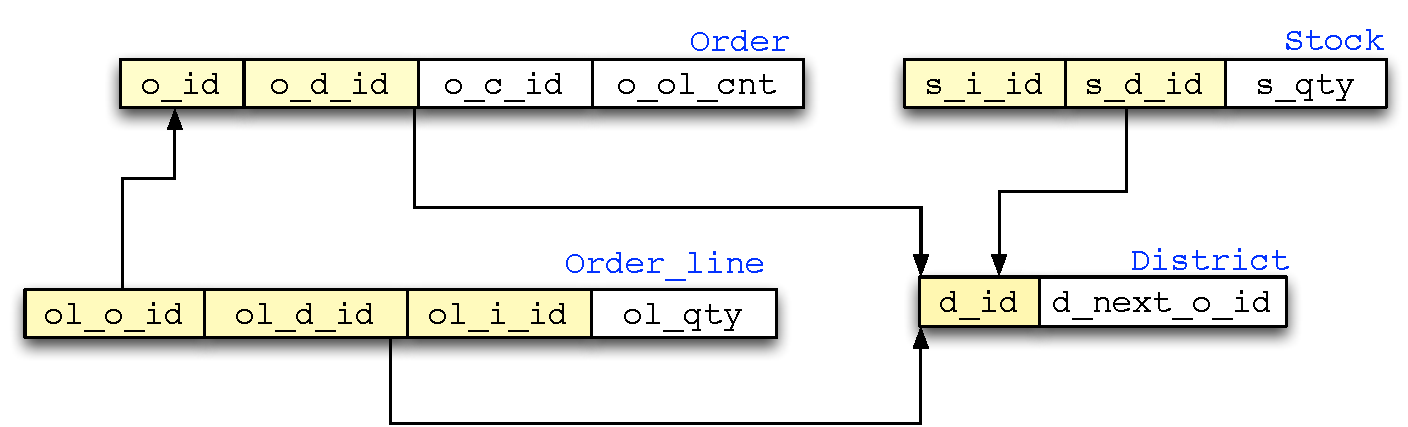
\includegraphics[scale=0.5]{Figures/schema}
\caption{Database schema of TPC-C's order management system.
  Columns against highlighted background are primary keys. Arrows denote
  foreign key relationships.}
\label{fig:schema}
\end{figure}

The \C{new\_order} transaction inserts a new \C{Order} record, whose
id is the sequence number of the next order under the given district
(\C{d\_id}). The sequence number is stored in the corresponding
\C{District} record, and updated each time a new order is added to the
system. Since each order may request multiple items (\C{item\_reqs}),
an \C{Order\_line} record is created for each requested item to relate
the order with the item. Each item has a corresponding record in the
\C{Stock} table, which keeps track of the quantity of the item left in
stock (\C{s\_qty}). The quantity is updated by the transaction to
reflect the processing of new order (if the stock quantity falls below
10, it is automatically replenished by 91).

TPC-C defines multiple invariants, called \emph{consistency
  conditions}, over the state of the application in the database. One
such consistency condition is the requirement that for a given order
\C{o}, the \emph{order-line-count} field (\C{o.o\_ol\_cnt}) should
reflect the number of order lines under the order; this is the number
of \C{Order\_line} records whose \C{ol\_o\_id} field is the same as
\C{o.o\_id}.  In a sequential execution, it is easy to see how this
condition is preserved.  A new \C{Order} record is added with its
\C{o\_id} distinct from existing order ids, and its \C{o\_ol\_cnt} is
set to be equal to the size of the \C{item\_reqs} set. The \C{foreach}
loop runs once for each \C{item\_req}, adding a new \C{Order\_line}
record for each requested item, with its \C{ol\_o\_id} field set to
\C{o\_id}. Thus, at the end of the loop, the number of \C{Order\_line}
records in the database, whose \C{ol\_o\_id} is equal to \C{o\_id} is
equal to the size of the \C{item\_req} set, which in turn is equal to
the \C{Order} record's \C{o\_ol\_cnt} field, thus preserving the
consistency condition.

Because the aforementioned reasoning is reasonably simple to perform
manually, verfiying the soundess of TPC-C's consistency conditions
would appear to be feasible.  Serializability aids the tractability of
verification by preventing any interference among concurrently
executing transactions while the \C{new\_order} transaction executes.
Under weak isolation\footnote{Weak isolation does not violate
  atomicity as long as the witnessed effects are those of committed
  transactions}, however, interferences of various kinds are
permitted.  Although the verification problem for weakly isolated
transactions would appear to be superficially similar to the
verification of (racy) concurrent programs (e.g., garbage
collectors~\cite{JLP+14,GHE15,HPQ+15}), weak isolation introduces new
challenges arising from the use of transactions, and new opportunities
arising from the fact that the store abstraction used by transactions
is a relational database, not low-level memory.

To illustrate some of these challenges, consider the behavior of the
\C{new\_order} transaction when executed with a \emph{Read Committed}
(RC) isolation level, the default isolation level in PostgreSQL, a
widely used open-source database system.  An RC transaction is
isolated from \emph{dirty writes}, i.e., writes of uncommitted
transactions, but is allowed to witness the writes of concurrent
transactions as soon as they are committed. Thus, with two concurrent
instances of the \C{new\_order} transaction (call them $T_1$ and
$T_2$), both concurrently placing new orders for different customers
under the same district (\C{d\_id}), PostgreSQL admits the two
executions shown in Fig.~\ref{fig:new_order_execs}.

\begin{figure}[!h]
\centering
\subcaptionbox {
  {\sc rc} Execution 1
  \label{fig:motiv-eg-1-b}
} [
  0.55\columnwidth
] {
  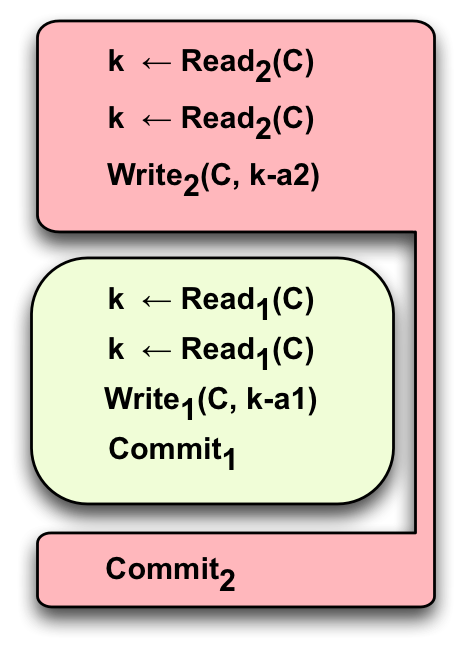
\includegraphics[scale=0.45]{Figures/motiv-eg-1-b}
}
%\hspace*{0.5in}
\subcaptionbox {
  {\sc rc} Execution 2
  \label{fig:motiv-eg-1-a}
}{
  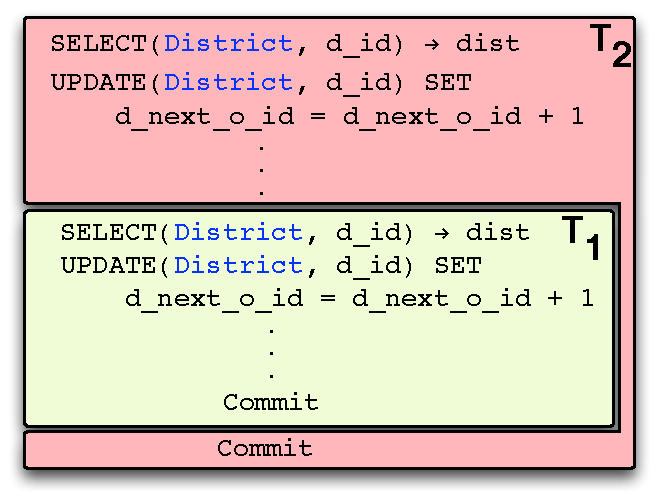
\includegraphics[scale=0.45]{Figures/motiv-eg-1-a}
}
  \caption{\small RC executions involving two instances ($T_1$ and
  $T_2$) of the \C{new\_order} transaction depicted in
  Fig.~\ref{fig:new_order_code}. 
  Each instance reads the \C{d\_id} \C{District} record twice, the second
  time to (atomically) update the \C{d\_next\_o\_id} field.}
\label{fig:new_order_execs}
\end{figure}

The figure depicts an execution as a series of transactional read, write, and commit
operations. In the execution on the left, the \C{new\_order} instance
$T_1$ (green) reads the \C{d\_next\_o\_id} field of the district
record for \C{d\_id}, but before it increments the field, another
\C{new\_order} instance ($T_2$) begins its execution and commits. Note
that $T_2$ reads the same \C{d\_next\_o\_id} value as $T_1$, and
inserts new \C{Order} and \C{Order\_line} records with their \C{o\_id}
and \C{ol\_o\_id} fields (resp.) equal to \C{d\_next\_o\_id}. $T_2$
also increments the \C{d\_next\_o\_id} field, which $T_1$ has already
acccessed. This is allowed because reads do not obtain a mutually
exclusive lock on most databases, including PostgreSQL. After $T_2$'s
commit, $T_1$ resumes execution and adds new \C{Order} and
\C{Order\_line} fields with the same order id as $T_1$. Thus, by the
end of the execution, \C{Order\_line} records inserted by $T_1$ and
$T_2$ all bear the same order id. There are also two \C{Order} records
with the same district id (\C{d\_id}) and order id, none of whose
\C{o\_ol\_cnt} reflects the actual number of \C{Order\_line} records
inserted with that order id.  This clearly violates TPC-C's consistency
condition.

Notably, this example does not exhibit any common concurrency bugs
that arise from incorrect use of weak isolation such as
\emph{write-write} conflicts, or \emph{lost updates}.  While $T_1$ and
$T_2$ both increment the \C{d\_next\_o\_id} field of the district
record, they do so atomically (Line 4 of
Fig.~\ref{fig:new_order_code}), allowing both updates to be present in
the final state. Likewise, other well-known anomalies that
characterize RC isolation~\cite{berenson} such as \emph{fuzzy reads},
\emph{phantom reads}, \emph{read skew}, and \emph{write skew}, are
also not exhibited by the example.  Thus, program analyses that aim to
determine appropriate isolation by checking for possible
manifestations of these anomalies would fail to identify grounds for
promoting the isolation level of \C{new\_order} to something stronger.
Yet, if we take the semantics of the application into account, it is
quite clear that RC is not an appropriate isolation level for
\C{new\_order}.

While reasoning in terms of anomalies is cumbersome, and as the above
example shows often inadequate, reasoning about weak isolation in
terms of low-level traces~\cite{adyaphd,gotsmanconcur15} complicates
high-level reasoning.  A possible alternative would interleave weak
isolation implementation details within the program, yielding a
(more-or-less) conventional concurrent program that can be then
subject to classical concurrent verification methods.  Considering the
size and complexity of real-world transaction systems, this strategy
is unlikely to scale.

In this paper, we adopt a different approach that \emph{lifts}
isolation semantics (\emph{not} their implementations) to the
application layer, providing a principled framework to simultaneously
reason about application invariants and isolation properties.  To
illustrate this idea informally, consider how we might verify that
\C{new\_order} is sound when executed under a \emph{Repeatable Read}
(RR) isolation level.  PostgreSQL executes an RR transaction by taking
a (conceptual) snapshot of the database state before the transaction
begins that is used by reads performing the transaction.  When the
transaction attempts to update a record, a check is made to determine
if the current version of the record in the database is the same as the
snapshot version. If it is, an exclusive lock is obtained on the
record, and the update is performed. If the record is already locked,
the transaction blocks until the lock is released.  When the lock is
obtained, is held exclusively until the transaction commits or rolls
back. If the aforementioned version check fails (i.e., the database
has a later version than the snapshot), the transaction is rolled back
and re-executed.

\begin{figure}[t]
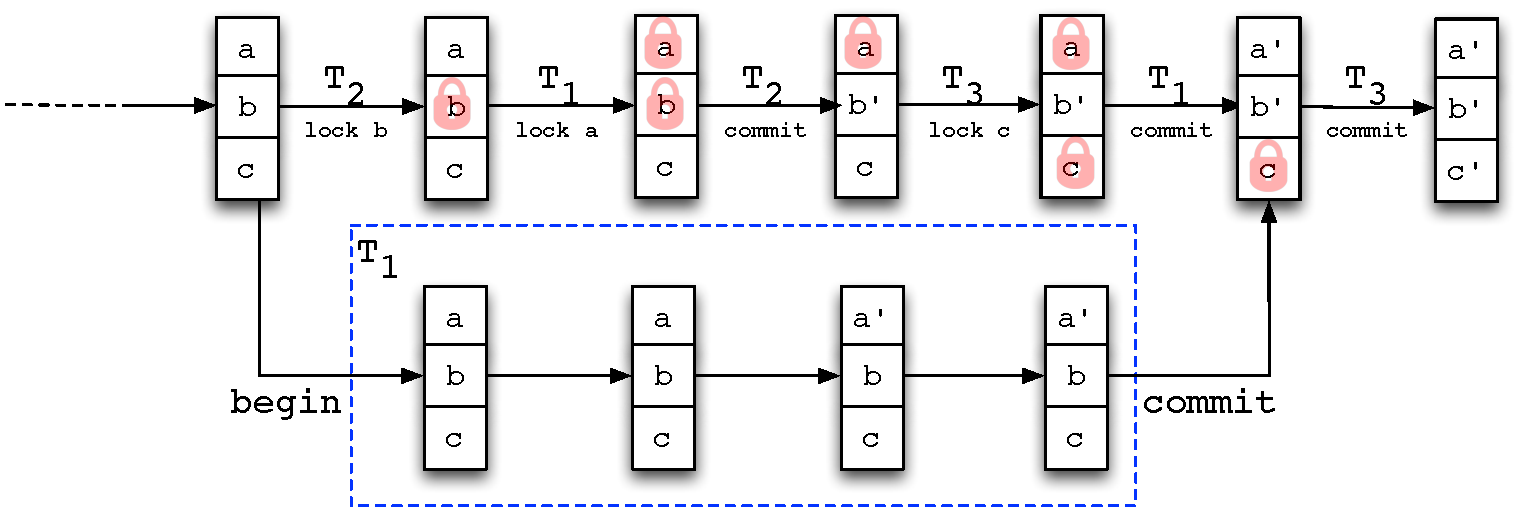
\includegraphics[scale=0.5]{Figures/RR-postgres}
\caption{Database state transitions corresponding to an execution of
  an RR transaction $T_1$ on PostgresSQL. $T_2$ and $T_3$ are concurrent
  transactions. The database state has three data items, $a$, $b$ and $c$. }
\label{fig:rr-postgres}
\end{figure}
\begin{figure}[t]
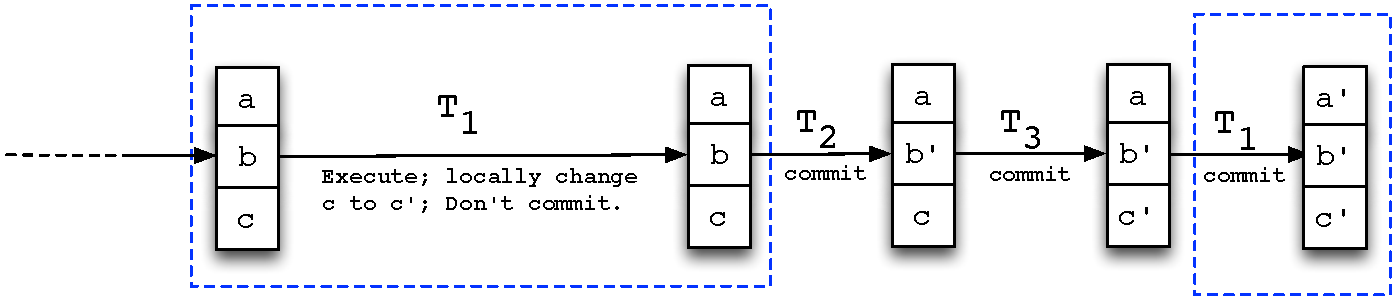
\includegraphics[scale=0.5]{Figures/RR-abstract}
  \caption{An abstract execution that includes the concrete execution
  shown in Fig.~\ref{fig:rr-postgres}. It has no locks or snapshots,
  admits fewer interleavings, yet results in the same post-state.  }
\label{fig:rr-abstract}
\end{figure}

Although this implementation, comprising many thousands of lines of
code, is highly involved, its semantic behavior in terms of how it
effects transitions on the database state is fairly simple.  Since a
transaction's reads are always served from a snapshot, no state
changes are witnessed while the execution is in progress. Thus,
insofar as an RR transaction is concerned, the database state does not
change during the execution.  Uncommitted writes are recorded in a
transaction-local state.  When the transaction commits, the local
state is atomically written to the global state to yield a global
state that reflects the transaction's updates.  However, unlike a
strongly isolated serializable transaction, the commit operation is
performed against the current state of the database, not the
snapshot. Thus, after the transaction finishes execution, but before
it commits, the transaction is able to witness the effects of all
concurrent transactions that committed before it.  The PostgreSQL RR
implementation effectively constrains this transition.

We can axiomatize this operational description by observing that (a)
due to the version check, the current transaction cannot update a data
item that was already updated by a concurrent transaction, and (b) due
to the use of exclusive write locks, a data item updated by the
current transaction cannot be overwritten by a concurrent transaction.
If $\Delta$ is the state of the database when an RR transaction
finishes, and $\Delta_c$ is the state visible to the transaction at
the point of commit, we know the transition from $\Delta$ to
$\Delta_c$ (written $\Delta \longrightarrow \Delta_c$) cannot exhibit
effects from any concurrent transactions that write to the same data
items as the current RR transaction.  Similarly, if $\delta$ denotes
a local log that relates transaction variables being written with their updated values,
then $\forall x\in\mathit{dom}(\delta)$, $\Delta_c(x) =
\Delta(x)$. To summarize, the operational semantics of PostgresSQL's RR
implementation can be captured as an axiomatization over transitions of
the database state ($\Delta \longrightarrow \Delta'$) during the
lifetime an RR transaction ($T$):
\begin{itemize}
  \item While $T$ executes, $\Delta' = \Delta$.
  \item After $T$ finishes execution, but before it commits its local
    state $\delta$, $\forall(x\in\delta).~\Delta'(x) = \Delta(x)$.
\end{itemize}

This simple characterization of RR isolation allows us to verify the
consistency condtions associated with the \C{new\_order}
transaction. First, since the database doesn't change ($\Delta' =
\Delta$) (where $\Delta'$ represents the state after the transaction
commits), during the execution of the transaction's body, we can
reason about \C{new\_order} as if it executed in complete isolation
until its commit point, leading to a verification process similar to
what would been applied when reasoning about serializability.  When
\C{new\_order} finishes execution and becomes ready to commit, a
transition that transfers the transaction'slocal writes ($\delta$) to
the unchanged database state ($\Delta$).  However, we are required to
consider the interference from concurrent transitions at this point,
which might change the database state from $\Delta$ to $\Delta_c$. If
this interference includes the effects of a concurrent \C{new\_order}
transaction (with the same \C{d\_id}), then verification fails as
described previously (Fig.~\ref{fig:new_order_execs}). Fortunately,
sequential reasoning shows that this is impossible - RR prevents a
concurrent \C{new\_order} transaction that modifies the same
\C{District} record as the current transaction (concretely, since the
record is already present in the current transaction's local log, any
transition from $\Delta$ to $\Delta_c$ cannot change this record).
Applying such axiomatic reasoning on \C{new\_order} allows us to prove
that the TPC-C invariant holds when the transaction is executed under
PostgreSQL's RR isolation.  Our proof framework generalizes this style
of reasoning to various isolation levels on databases.

The second observation that informs our approach is one that pertains
to automation. Program verification, even when machine-aided, often
entails significant annotation burden in the form of intermediary
assertions and loop invariants required to prove a program correct.
This is certainly true for concurrent program logics, such as
Rely-Gurantee, which extend Hoare logic with additional artifacts and
where (stable) intermediary assertions and loop invariants remain a
major source of annotation burden.  However, a relational database is
a significantly simpler abstraction than shared memory. There are no
pointers, or linked data structures, or aliasing.  Although a database
essentially abstracts a mutable state, the state is mutated through a
well-defined fixed number of interfaces (SQL statements), each tagged
with a logical formula describing what records are accessed and
updated. 

This observation leads us away from thinking of database transactions
as concurrent imperative programs.  Instead, we see value in viewing
them as essentially functional computations that manage database state
monadically. We find it useful to reason about
statements that mutate the database state, not in terms of a pre- and
post-condition pair, but in terms of a state transformer that relates
the pre- and post-states of a statement. This state transformer
semantics can be defined algorithmically, just like predicate
transformer semantics (e.g., strongest post-condition).  Here, a state
transformer interprets a SQL statement in the set domain, taking
advantage of the fact that a a database is essentially a set of
tuples, and a SQL statement is a transformer over these sets.  The
benefit of this approach is that low-level loops can now be
substituted with higher-order combinators that automatically lift the
state transformer of its higher-order argument (i.e., the loop body)
to the state transformer of the combined expression (i.e., the loop).
Thus the semantics of a \C{foreach} loop, for instance, can be
captured as a state transformer, where the state is a set, and the
transformation defines a bind operation. We illustrate this intuition
on a simple example.

% \begin{figure}[!t]
% \centering
% %
% \begin{subfigure}[b]{0.46\textwidth}
% \begin{ocaml}
% Set s' = $\emptyset$;
% foreach x in s {
%   s'.add(f(x)); 
% }
% \end{ocaml}
% \caption{}
% \end{subfigure}
% %
% \begin{subfigure}[b]{0.5\textwidth}
% \begin{ocaml}
% let s' = ref [];
% foreach s (fun x -> s' := x::(!s'));
% \end{ocaml}
% \caption{Lorem ipsum, lorem ipsum,Lorem ipsum, lorem ipsum,Lorem ipsum}
% \end{subfigure}
% \caption{Caption place holder}
% %
% \caption{New versions are created from existing versions either
% through \C{push} or \C{merge}.}
% \label{fig:syntactic-ancestors}
% \end{figure}
% let s' = ref (Set.empty) in
% foreach xs @@ fun x -> 
%   begin
%     s' := Set.union !s' @@ 
%             Set.map_selected s (fun y -> y<x)
%                                (fun y -> y+x);
%     s' := Set.add !s' x;
%   end
\begin{figure}[!h]
\begin{ocaml}
foreach item_reqs @@ fun item_req -> do
  SQL.update Stock (fun s -> {s with s_qty = k1}) 
                   (fun s -> s.s_i_id = item_req.ol_i_id);
  SQL.insert Order_line {ol_o_id=k2; ol_d_id=k3; 
                         ol_i_id=item_req.ol_i_id; ol_qty=item_req.ol_qty}
\end{ocaml}
\caption{Foreach loop from Fig.~\ref{fig:new_order_code}}
\label{fig:foreach_code}
\end{figure}

Fig.~\ref{fig:foreach_code} shows a (simplified) snippet of code taken
from Fig.~\ref{fig:new_order_code}. Some irrelevant expressions have
been replaced with constants (\C{k1} to \C{k3}).  The body of the loop
executes a SQL update followed by an insert.  Recall that a transaction
reads from the global database ($\Delta$), and writes to a
transaction-local database ($\delta$) before committing these updates. An update
statement filters the tuples that match the search criteria from $\Delta$
and computes the updated tuples that are to be
added to the local database. Thus, its state transformer (call it
$T_U$) is the following function on sets\footnote{$\bind$ has higher precedence than $\cup$.}:
\begin{ocaml}
  fun ($\Delta$,$\delta$) -> $\delta$ $\cup$ $\Delta$$\bind$(fun s -> if table(s) = stock && s.s_i_id = item_req.ol_i_id 
                                 then {{s with s_qty = k1}} (* a singleton set *)
                                 else $\emptyset$)
\end{ocaml}
% \begin{smathpar}
% \begin{array}{c}
%   \lambda\Delta.\lambda\delta.\, \delta \;\cup\; 
%       \Delta \,\bind\, (\lambda s.\, 
%           \C{if}\;{\C{stock}(s) \conj 
%                    \C{s.s\_i\_id} = \C{item\_req.ol\_i\_id}}\\
%            \hspace*{0.9in}
%            \C{then}\;{\{\{s \;\C{with}\; \C{s\_qty} = \C{k1}\}\}}\;
%            \C{else}\;{\emptyset})
% \end{array}
% \end{smathpar}
% \begin{verbatim}
%   Rmem(σ'(s')) = Rmem(σ(s')) U 
%                  Rmem[\x. Rmem[\y. if y<x then {y+x} else {}](σ(s)) U {x}](xs)
% \end{verbatim}
Observe that
$T_U(\Delta,\delta)$ is of the form $\delta \,\cup\,
F_U(\Delta)$. The transformer ($T_I(\Delta,\delta)$)
for the subsequent \C{insert} statement can be similarly calculated to
be of the form $\delta \cup F_I(\Delta)$.
Their composition gives the state transformer of the loop body:
\begin{ocaml}
  fun ($\Delta$,$\delta$) -> $\delta$ $\cup$ $F_U(\Delta) \,\cup\, F_I(\Delta)$
\end{ocaml}
Let $F_{body}(\Delta) = F_U(\Delta) \,\cup\, F_I(\Delta)$.   The
transformer for the \C{foreach} loop can now be computed as following:
\begin{ocaml}
  fun ($\Delta$,$\delta$) -> $\delta$ $\cup$ item_reqs$\bind$(fun item_req -> $F_{body}(\Delta)$)
\end{ocaml}
Observe that the transformer captures the precise semantics of the
loop as a formula in the domain of sets extended with a bind
function. The advantage in doing so is that we can now make use of a
semantics-preserving translation from this domain to first-order
logic, allowing us to leverage SMT solvers for automatic proofs
without having to infer loop invariant, or provide intermediate
assertions.  Sec.~\ref{sec:automation} describes this translation. In
the exposition thus far, we assumed $\Delta$ remains invaraint, which
is clearly not the case when we admit concurrency.  Necessary
concurrency extensions of the state transformer semantics is also
covered in Sec.~\ref{sec:automation}.  The following two sections,
however, focus on laying theoretical foundations for reasoning about
weak isolation.


\section{\txnimp: Syntax and Semantics}
\label{sec:opsem}

\label{sec:syntax}

\renewcommand{\ctxn}[3]{\C{TXN}_{#1}\langle #2 \rangle\{#3\}}
\begin{figure*}[!ht]
\raggedright
%
\textbf{Syntax}\\
%
\begin{smathpar}
\renewcommand{\arraystretch}{1.2}
\begin{array}{lclcl}
\multicolumn{5}{c} {
  {x,y} \in \mathtt{Variables}\qquad
  {f} \in \mathtt{Field\;Names} \qquad
% {\tau} \in \mathtt{Table\;Names}
  {i,j} \in \mathbb{N} \qquad
  {\odot} \in \{+,-,\le,\ge,=\}\qquad
}\\
\multicolumn{5}{c}{
  {k} \in \mathbb{Z}\cup\mathbb{B} \qquad
  {\rec} \in \{\bar{f}=\bar{k}\}\qquad
  {\stl,\stg,s} \in \Pow{\rec} \qquad
  \I \in \mathbb{B}\times\Pow{\rec}\times\Pow{\rec}\times\Pow{\rec}
  \rightarrow \Prop
}\\
v & \in & \mathtt{Values} & \coloneqq & k \ALT \rec \ALT s\\
e & \in & \mathtt{Expressions} & \coloneqq & c \ALT x \ALT x.f 
    \ALT \{\bar{f}=\bar{e}\} \ALT e_1 \odot e_2\\ 
c & \in & \mathtt{Commands} & \coloneqq & \cskip \ALT \lete{x}{e}{c}
    \ALT \ite{e}{c_1}{c_2}\ALT c_1;c_2 \ALT \inserte{e}  \\
&&&&\ALT \deletee{\lambda x.e}
    \ALT \lete{x}{\selecte{\lambda x.e}}{c}
    \ALT \updatee{\lambda x.e_1}{\lambda x.e_2}\\
&&&&\ALT \foreache{e_1}{\lambda x.\lambda y. e_2} 
    \ALT \foreachr{s_1}{s_2}{\lambda x.\lambda y. e}\\
&&&&\ALT \ctxn{i}{\I}{ c } \ALT \ctxn{i}{\I,\stl,\stg}{c} \ALT c1 || c2\\
% t & \in & \mathtt{Terms} & \coloneqq & e \ALT c\\
\ectx & \in & \mathtt{Eval\;Ctx} & ::= & \bullet \ALT  
  \bullet || c_2 \ALT c_1 || \bullet \ALT \bullet;\,c_2 
  \ALT \ctxn{i}{\I,\stl,\stg}{\bullet} \\
\end{array}
\end{smathpar}
%
\bigskip

\renewcommand{\arraystretch}{1.2}

%
\textbf{Local Reduction} \quad 
\fbox {\(\stg \vdash (c,\stl) \stepsto (c',\stl')\)}\\
%
\begin{minipage}{2.8in}
\rulelabel{E-Insert}
\begin{smathpar}
\begin{array}{c}
\RULE
{
  i \not\in \dom(\stl \cup \stg)\\
  r = \{\bar{f}=\bar{k};\,\idf=i;\,\delf=\C{false}\}
}
{
  \stg \vdash (\inserte{\{\bar{f}=\bar{k}\}},\stl) \stepsto
  (\cskip,\stl \cup \{r\})
}
\end{array}
\end{smathpar}
\end{minipage}
%
%
\begin{minipage}{2.8in}
\rulelabel{E-Delete}
\begin{smathpar}
\begin{array}{c}
\RULE
{
  s = \{r' \,|\, \exists(r\in\Delta).~ \eval([r/x]e)=\C{true} \\
        \hspace*{0.7in}\conj r'=\{\bar{f}=r.\bar{f}; \idf=r.\idf;
        \delf=\C{true}\}\}\\
% \dom(s) \cap \dom(\delta) = \emptyset
}
{
  \stg \vdash (\deletee{\lambda x.e},\stl) \stepsto (\cskip,\stl \cup s)
}
\end{array}
\end{smathpar}
\end{minipage}
%
\bigskip

%
\begin{minipage}{2.8in}
\rulelabel{E-Select}
\begin{smathpar}
\begin{array}{c}
\RULE
{
  s = \{r\in\Delta \,|\, \eval([r/x]e)=\C{true}\}\spc
  c' = [s/x]c
}
{
  \stg \vdash (\lete{x}{\selecte{\lambda x.e}}{c}, \stl) \stepsto 
              (c',\stl)
}
\end{array}
\end{smathpar}
\end{minipage}
%
%
\begin{minipage}{2.8in}
\rulelabel{E-Update}
\begin{smathpar}
\begin{array}{c}
\RULE
{
  s = \{r' \,|\, \exists(r\in\Delta).~ \eval([r/x]e_2)=\C{true} \conj r'=[r/x]e_1\}\\
}
{
  \stg \vdash (\updatee{\lambda x.e_1}{\lambda x.e_2},\stl) \stepsto 
              (\cskip,\stl \cup s)
}
\end{array}
\end{smathpar}
\end{minipage}
%

\begin{smathpar}
\begin{array}{ll}
  \rulelabel{E-Foreach1} & \stg \vdash (\foreache{e}{\lambda x.\lambda
  y.c},\stl) \stepsto (\foreachr{\emptyset}{\eval(e)}{\lambda x.\lambda y. c})\\
  \rulelabel{E-Foreach2} & \stg \vdash (\foreachr{s_1}{\{r\} \cup s_2}{\lambda x.\lambda
  y.c},\stl) \stepsto ([r/y][s_1/x]c;\,\foreachr{s_1 \cup \{r\}}{s_2}{\lambda x.\lambda y. c})\\
  \rulelabel{E-Foreach3} & \stg \vdash (\foreachr{s}{\emptyset}{\lambda x.\lambda
  y.c},\stl) \stepsto (\cskip,\stl)\\
\end{array}
\end{smathpar}
%
\bigskip

%
\textbf{Top-Level Reduction} \quad 
\fbox {\((c,\stg) \stepsto (c',\stg')\)}\\
%
\begin{minipage}{3in}
\rulelabel{E-Txn}
\begin{smathpar}
\begin{array}{c}
\RULE
{
  \I(\C{true},\stl,\stg,\stg')\spc
  \stg \vdash (c,\stl) \stepsto (c',\stl')
}
{
  (\ctxn{i}{\I,\stl,\stg}{c},\stg') \stepsto
  (\ctxn{i}{\I,\stl',\stg'}{c'},\stg')
}
\end{array}
\end{smathpar}
\end{minipage}
%
%
\begin{minipage}{2.8in}
\rulelabel{E-Commit}
\begin{smathpar}
\begin{array}{c}
\RULE
{
  \I(\C{false},\stl,\stg,\stg')
}
{
  (\ctxn{i}{\I,\stl,\stg}{\cskip},\stg') \stepsto (\cskip,\stl\gg\stg')
}
\end{array}
\end{smathpar}
\end{minipage}
%


\caption{\small \txnimp: Syntax and Small-step semantics}
\label{fig:txnimp}
\end{figure*}



Fig.~\ref{fig:txnimp} shows the syntax and small-step semantics of
\txnimp, a core language that we will use to formalize the intuitions
presented in the previous section. Natural numbers, (shared) variables
and arithmetic expressions constitute the syntactic class of
expressions ($e$).  Commands ($c$) include $\cskip$, assignment
statements, transaction (\C{txn}) lexical blocks, and their sequential
and parallel composition. We let $T_i$ for $i \in \mathbb{N}$ range
over transaction identifiers. When it is evident we are referring to a
transaction, we use the number $i$ instead of $T_i$ for identification
(\eg in $\C{txn}\langle i \rangle$). Like variables, transaction
identifiers are globally accessible. For notational convenience, we
let $t$ range over both expressions and commands.

We define a small-step operational semantics for this language in
terms of an abstract machine that generates an execution trace ($\E$).
The first component of the trace is a set ($\A$) of \emph{effects},
where an effect ($\eta$) is a tuple of (a). the identifier ($T_i$) of
the transaction that generated this effect, (b). the unique
identifier ($j$) of this effect, (c). the operation ($\op$)
documented by this effect, which can be either a read (\C{RD(X)}), a
write (\C{WR(X)}), or a transaction commit (\C{COMMIT}), and (d). the
value, if any, associated with the operation (\eg, value read or value
written). Functions $\txn$, $\id$, $\oper$, and $\rval$ project each
of the four aforementioned individual components of the tuple.  In
every step of the evaluation, the machine reduces a \txnimp\ term by
executing a read, write or commit operation, generating an effect, and
extending the trace. Since effects include transaction identifiers,
the semantics distinguishes between terms ($t$) of different
transactions. For example, $\txnbox{t}_i$ denotes a term $t$ inside a
transaction $T_i$.  Evaluation contexts are also appropriately marked.
For example, $\ectx_i$ denotes the evaluation context for a term
inside $T_i$. The other component of an execution trace is a
visibility relation ($\visZ$) that establishes a visibility property
between effects among different transactions. The intent and mechanics
of $\visZ$ is described in the sequel.

Fundamental to our development is the notion of a trace invariant
($\I$). $\I$ is a function from traces ($\E$) to first-order logical
formulas ($\Prop$) that define well-formedness
constraints over traces.  The machine takes a step only if the
resulting trace satisfies the constraints imposed by $\I$. This
behaviour is captured by the auxiliary reduction rule
\rulelabel{E-Aux} that factors out the trace extension aspect of the
evaluation by abstracting away the operation-specific behaviour as a
function that generates an appropriate effect. We let $\mathcal{F}$
denote this function.  \rulelabel{E-Aux} uses $\mathcal{F}$ to
generate a new effect and extend the trace ($\E = (\A,\visZ)$)
\emph{only if} the well-formedness constraints imposed by $\I$ on $\E$
(i.e., $\I(\E')$) are satisfied. Otherwise, it gets stuck. In an
execution that runs to completion, every small-step preserves the
well-formedness of a trace, thus ensuring the invariance of $\I$.
Note that the semantics makes no assumptions about $\I$ other than its
type. As such, it can be instantiated with any trace-parametric
proposition that expresses constraints over the given trace. For
instance, consider the $\psi_{RC}$ specification from
\S\ref{sec:motivation}, but with bounded $T_1$ and $T_2$ instantiated
with \C{Wd1} and \C{Wd2}, respectively. The instantiated specification
is the following term:\vspace*{-8pt}

\begin{smathpar}
\begin{array}{l}
  \forall \eta_1,\eta_2.\; \txn(\eta_1) = \C{Wd1}
  \conj \txn(\eta_2) = \C{Wd2} \\
  \hspace*{0.6in}\conj \C{Wd1} \neq \C{Wd2} \conj \eta_1 \hboar
  \eta_2 \Rightarrow \C{Wd1} \hboar \eta_2 \\
\end{array}
\end{smathpar}

\noindent It is easy to interpret the above specification in the
context of a trace $\E$ that captures an execution of the program in
Fig.~\ref{fig:motiv-eg-1}. Such a trace-parametric formula can be
used to instantiate the trace invariant $\I$ in Fig.~\ref{fig:txnimp}.
The resultant operational semantics describes an abstract machine that
gets stuck if an operation of \C{Wd2} is executed in a state that
incorporates some, but not all the effects (including the \C{COMMIT})
of \C{Wd1}.
% While the machine takes a step only if the constraints are
% satisfied, it neither defines nor explicitly assumes an oracle to
% check satisfaction.

As described in \S\ref{sec:motivation}, the semantics of various
isolation levels can be captured as constraints over the
happens-before ($\hbZ$) relation. $\hbZ$ is however a derived relation
in our model, composed of more fundamental \emph{session order}
($\soZ$) and \emph{visibility} ($\visZ$) relations. In particular,
$\hbZ \,=\, (\soZ \cup \visZ)^{+}$. Unlike $\hbZ$, $\visZ$ (defined
below) is not a transitive relation, and hence lets us capture
finer-grained isolation properties than $\hbZ$, which we leverage in
our development.  The session order relation captures the sequential
order of operations within a transaction. In particular, it relates
two effects, $\eta_1$ and $\eta_2$, such that $\txn(\eta_1) =
\txn(\eta_2)$ and $\id(\eta_1) < \id(\eta_2)$.  The semantics assigns
monotonically increasing identifiers to effects, as defined by the
$\id(\eta) > \maxId(\A)$ condition of \rulelabel{E-Aux} ($\maxId(\A)$
returns the maximum number identifying an effect in $\A$). Evaluation
contexts ($\ectx_i$) for transaction-bound terms are defined so as to
enforce a deterministic sequential order of execution within a
transaction, leading to a deterministic total order among effect ids,
which defines the session order relation. Visibility ($\visZ$) on the
other hand relates effects across concurrent transactions.
Intuitively, $\visZ$ relates $\eta_1$ to $\eta_2$ if and only if
$\eta_1$ was \emph{visible} to the operation that generated $\eta_2$
during its execution, thus effecting its return value
($\rval(\eta_2)$). For example, a read operation over \C{X} may pick
the value ($\rval$) of the write effect with the highest id among its
visible effects (this is made possible by appropriately defining
$\interp{\cdot}$ in \rulelabel{E-Var}, as we show later). Thus, the
value of a read depends on what write effects it can witness. An
operation can only witness the effects of already concluded
operations, which varies between executions due to the
non-deterministic order of evaluating the parallel composition of
transactions.

A more notable source of non-determinism, however, is the
\rulelabel{E-Aux} rule, which allows the machine to expose an
arbitrary subset ($S$) of existing effects ($\A$) to the incoming
operation. In other words, the machine is not obligated to reveal the
effects of all previous operations to an incoming operation. This
relaxation allows the abstract machine to model the semantics of
weakly-consistent data stores. For instance, operations issued to an
eventually consistent ({\sc ec}) replicated store could be dispatched
to different replicas whose states may not be in any well-defined
relationship. By allowing operations to witness arbitrary subsets of
the global state, the semantics models the weak visibility properties
of such stores; we elaborate on the implication of this style of
definition in \S\ref{sec:store-consistency}.  Stronger visibility
properties can be expressed by imposing well-formedness constraints
over $\visZ$ via the trace invariant ($\I$). Since the abstract
machine is obligated to satisfy $\I$ at every step of the execution,
operations are guaranteed to experience the level of isolation
specified by $\I$.  Thus, in executions that run to completion, the
abstract machine models a store that provides the required levels of
isolation.  Notably, the machine achieves this without defining an
operational semantics for isolation levels, instead solely relying on
their declarative characterization as trace well-formedness
constraints to enforce isolation guarantees.
\S\ref{sec:ansi-isolation} specifies various ANSI SQL isolation levels
stated as trace well-formedness constraints.

% TRACE RELATIONS
% ---------------
\begin{figure*}[t!]
\begin{minipage}{\columnwidth}
\begin{smathpar}
\begin{array}{lcl}
(\A,\visZ) \Vdash \eta \in T_i & \defeq & \eta \in \A \conj \txn(\eta) = T_i\\
\E \Vdash S \subseteq T_i & \defeq & \forall \eta.~ \eta
        \in S \Rightarrow \underE{\eta \in T_i} \\
(\A,\visZ) \Vdash \eta_1 \visar \eta_2 & \defeq & \{\eta_1,\eta_2\}
        \subseteq \A \conj (\eta_1,\eta_2) \in \visZ\\
(\A,\visZ) \Vdash \eta_1 \soar \eta_2 & \defeq & \{\eta_1,\eta_2\}
        \subseteq \A \conj \txn(\eta_1)=\txn(\eta_2) \\
        &   & \hspace*{0.3in} \conj \id(\eta_1) < \id(\eta_2)\\
\E \Vdash T_i \visar \eta & \defeq &\forall\eta_1
        .\,(\E \Vdash \eta_1 \in T_i) \Rightarrow \E \Vdash \eta_1 \visar \eta \\
\end{array}
\end{smathpar}
\end{minipage}
\begin{minipage}{\columnwidth}
\begin{smathpar}
\begin{array}{lcl}
\underE{T_i \visar T_j} & \defeq &  \forall\eta_1,\eta_2.\,
    %\sameobj{\eta_1}{\eta_2}  \Rightarrow 
    \underE{\eta_1\in T_i} \conj \underE{\eta_2 \in T_j} \\
    &   & \hspace*{1in}\Rightarrow \underE{\eta_1 \visar \eta_2} \\
\underE{T_i \invisar T_j} & \defeq &  \forall\eta_1,\eta_2.\,
        %\sameobj{\eta_1}{\eta_2}\Rightarrow 
        \underE{\eta_1\in T_i} \conj \underE{\eta_2 \in T_j}\\
    &   & \hspace*{1in} \Rightarrow \neg (\underE{\eta_1 \visar \eta_2})\\
\underE{T_i \wrstoar X} & \defeq & \exists\eta.~
        \underE{\eta \in T_i} \conj \kind(\eta) = \C{WR}(X)\\
\underE{T_i \rdsfmar X} & \defeq & \exists\eta.~
        \underE{\eta \in T_i} \conj \kind(\eta) = \C{RD}(X)\\
\underE{T_i \usesar X} & \defeq & \underE{T_i \wrstoar X} \disj
      \underE{T_i \rdsfmar X}\\
\end{array}
\end{smathpar}
\end{minipage}

\caption{Relations defined over a trace}
\label{fig:rel-defs}
\end{figure*}




% However, a machine that lets operations witness arbitrary subset of
% the global state offers no isolation whatsoever. For example, it may
% allow a read operation to witness writes of an uncommitted
% transaction, violating RC isolation. Fortunately, our ability to
% express an isolation semantics as constraints over happens-before
% order through $\visZ$ and $\soZ$ relations, and the property of the
% abstract machine to be parametric over the trace invariant ($\I$),
% lets us solve this problem.
% In particular, we continue to define isolation semantics as
% constraints over $\visZ$ and $\soZ$, but confine their domain of
% interpretation to the given trace so that they now become trace
% well-formedness constraints. Well-formedness constraints can be
% combined into a trace invariant ($\I$). 


As described previously, \rulelabel{E-Aux} abstracts away the
operation-specific behaviour of a machine step as a function ($\F$)
that accepts a set ($S$) of effects chosen by the machine to make
visible to the operation, interprets the operation w.r.t. $S$, and
returns an appropriate effect that encodes its return value. Rules
\rulelabel{E-Var}, \rulelabel{E-Asgn} and \rulelabel{E-Commit} define
such functions for read, write and commit operations, respectively.
The effect returned by the function in each case includes its
transaction id ($T_i$) along with an arbitrarily chosen effect id
($j$) that is later verified to be unique in \rulelabel{E-Aux}. The
$\rval$ for a write is the value being written, and for commit it is
$\bot$. In case of a read, the value read depends on how the read
operation chooses to interpret the given set ($S$) of visible effects.
The interpretation may depend on application semantics. For example, a
monotonically increasing counter application may choose to let a write
with the largest value determine the value of a read. To accommodate
multiple interpretations, the semantics is made parametric over an
interpretation function ($\interp{\cdot}$) that accepts a set of
effects and a variable name, and returns the value associated with the
variable. A straightforward interpretation function that chooses the
last write (i.e., write with largest id) is shown below:

\begin{smathpar}
\begin{array}{lcl}
  \isMax(S,\eta) & \Leftrightarrow &  \forall (\eta'\in S).  
  \kind(\eta') = \kind(\eta) \\
  & & \hspace*{0.4in}\Rightarrow \eta' = \eta \disj \id(\eta') < \id(\eta)\\

\interp{S}(X) & = & \C{if}\;(\exists (\eta \in S). \kind(\eta) = \C{WR}(X) 
  \wedge \isMax(S,\eta)) \\
  & & \C{then}\;\rval(\eta)\;\C{else}\;0\\
\end{array}
\end{smathpar}

\noindent Rules \rulelabel{E-Top-Ctx} and \rulelabel{E-Txn-Ctx} define
congruence properties for top-level terms and transaction-bound terms,
respectively. The rules and evaluation contexts ($\ectx$ and
$\ectx_i$) are defined such that only certain kinds of terms are
allowed at the top-level and inside a transaction. In particular, a
\txnimp program at the top-level can either be a transaction, or a
parallel composition of transactions. A command inside a \C{txn} block
can either be an assignment, or a sequential composition of
assignments. 

\subsection{Specifications}
\label{sec:ansi-isolation}


% ISOLATION SPECS
% ---------------
\begin{figure*}[t!]
\begin{smathpar}
\begin{array}{lcl}
\underE{\C{RMWVis}(T_j)} & \defeq & \forall\eta_1,\eta_2.\,
       \underE{\{\eta_1,\eta_2\} \subseteq T_j} \conj
       \underE{\eta_1 \soar \eta_2} \Rightarrow \underE{\eta_1 \visar
       \eta_2}\\
\underE{\C{MonotonicVis}(T_j)} & \defeq & 
       \underE{\C{RMWVis}(T_j)} \conj 
       \forall\eta,\eta_1,\eta_2.\, \underE{\{\eta_1,\eta_2\} \in T_j} 
          \conj \\
  &   & \hspace*{1.2in}\underE{\eta \visar \eta_1} \conj
        \underE{\eta_1 \soar \eta_2} \Rightarrow \underE{\eta \visar
        \eta_2} \\
%  \C{CausalVis}(T_i) & \defeq & 
%         \C{MonotonicVis}(T_i) \conj \C{RMWVis}(T_i)\\
\underE{\C{AtomicVis}(T_j)} & \defeq & 
       \forall\eta_1,\eta_2.\, \neg(\underE{\eta_1 \in T_j}) \conj
       \underE{\eta_2 \in T_j} \conj
       \underE{\eta_1 \visar \eta_2} \Rightarrow \underE{\txn(\eta_1)
       \visar \eta_2}\\
\underE{\C{CommitVis}(T_j)} & \defeq & 
       \forall\eta_1,\eta_2.~ \neg(\underE{\eta_1 \in T_j}) \conj 
          \underE{\eta_2 \in T_j} \conj
       \underE{\eta_1 \visar \eta_2} \Rightarrow\\
  &   & \hspace*{1.2in}\exists\eta.\, \underE{\eta \in \txn(\eta_1)} 
        \conj \kind(\eta) = \C{COMMIT} 
        \conj \underE{\eta \visar \eta_2}\\
% \underE{\C{TransVis}(T_j)} & \defeq &  \forall
%        \eta_1,\eta_2,\eta_3.\, \underE{\eta_3 \in T_j} \conj
%        \underE{\eta_1 \visar \eta_2} \conj
%        \underE{\eta_2 \visar \eta_3} \Rightarrow \underE{\eta_1 \visar
%        \eta_3} \\
\underE{\C{RC}(T_j)} & \defeq & \underE{\C{AtomicVis}(T_j)} 
        \conj \underE{\C{CommitVis}(T_j)}\\
\underE{\C{MAV}(T_j)} & \defeq & \underE{\C{RC}(T_j)} \conj
      \underE{\C{MonotonicVis}(T_j)} \\
\underE{\C{SnapshotVis}(T_i,T_j)} & \defeq &  \underE{T_i
       \visar T_j} \disj \underE{T_i \invisar T_j}\\
\underE{\C{RR}(T_j)} & \defeq & \underE{\C{MAV}(T_j)}
       \conj \forall T_i.\,T_i \neq T_j \Rightarrow 
        \underE{\C{SnapshotVis}(T_i,T_j)} \\
% &   & \hspace*{2in}\conj  \C{SnapshotVis}(T_i,T_j)\\
\underE{\C{SnapshotSER}(T_i,T_j,X)} & \defeq &  \underE{T_i
       \visar T_j} \disj (\underE{T_i \invisar T_j} \conj \\
  &   &\hspace*{1.2in}\exists \eta.~\underE{\eta\in T_i} \conj \kind(\eta) =
       \C{WR(X)} \Rightarrow \underE{T_j \visar \eta})\\
\underE{\C{SI}(T_j)} & \defeq &  \underE{\C{RR}(T_j)}
       \conj \forall T_i.\,(T_i \neq T_j \conj \exists X.\, \underE{T_i \wrstoar X} \conj 
        \underE{T_j \wrstoar X})\\
%      (\exists X.\, T_i \wrstoar X \conj T_j \wrstoar X)
%      \Rightarrow  \C{TotalVis}(T_i,T_j)\\
  &   & \hspace*{2in} \Rightarrow \underE{\C{SnapshotSER}(T_i,T_j,X)}\\
\underE{\C{SER}(T_j)} & \defeq & \underE{\C{RR}(T_j)}
        \conj \forall T_i.\,(T_i \neq T_j \conj \exists X.\, 
        \underE{T_i \wrstoar X} \conj \underE{T_j \usesar X})\\
  &   & \hspace*{2in} \Rightarrow \underE{\C{SnapshotSER}(T_i,T_j,X)}\\
\end{array}
\end{smathpar}

\caption{Standard isolation guarantees expressed as trace
well-formedness constraints}
\label{fig:ansi-isolation}
\end{figure*}




We now describe specifications of standard isolation guarantees
expressed as constraints over trace well-formedness. For brevity and
convenience, we introduce some notations that are used in the following
sections.  An execution trace is destructed as ($\A$,$\visZ$) whenever
individual components of the pair are needed. Otherwise, it is written
as $\E$.  Sometimes, the dot notation (\eg~$\E.\A$) is also
used. Since $\A$ and $\visZ$ are both sets, we lift the operations on
sets to pairs of sets when updating $\E$. For example, $\E' = \E \cup
(\{\eta_2\},\{(\eta_1,\eta_2)\})$ expands to $\E' = (\E.\A \cup
\{\eta_2\},\,\E.\visZ \cup \{(\eta_1,\eta_2)\})$.  When $\psi$ is a
formula, $\underE{\psi}$ denotes the interpretation of $\psi$ in the
context of the trace $\E$. Such interpretations are defined on a
case-by-case basis in Figs.~\ref{fig:rel-defs}
and~\ref{fig:ansi-isolation}.

\subsubsection{Trace Relations}

Fig.~\ref{fig:rel-defs} shows various relations defined over elements
in a trace. In the context of a trace $(\A,\visZ)$, an effect $\eta$
is said to belong to a transaction $T_i$ if $\eta$ belongs to the
effect set $A$ and its transaction identifier is $T_i$. The
containment relation is trivially lifted to the set of effects to
define $\underE{S \subseteq T_i}$.  Visibility, session order, and
happens-before relations are denoted by $\eta_1 \visar \eta_2$,
$\eta_1 \soar \eta_2$, and $\eta_1 \hboar \eta_2$, respectively. A
transaction $T_i$ is said to be visible to an effect $\eta$ if every
effect $\eta_1$ of $T_i$ recorded by the trace is visible to $\eta$.
$T_i$ may be visible to $\eta$ but may not be visible to every other
effect in the $\txn(\eta)$. For a transaction $T_i$ to be considered
to be visible to a transaction $T_j$ in the context of a trace $\E$
(written $\underE{T_i \visar T_j}$), every effect ($\eta_1$) of $T_i$
present in $\E$ must be visible to every effect ($\eta_2$) of $T_j$ in
$\E$.  Conversely, if none of the effects of $T_i$ present in $\E$ are
visible to any effect of $T_j$, then $T_i$ is considered invisible to
$T_j$ under $\E$ (written $\underE{T_i \invisar T_j}$). Transaction
$T_i$ is said to have written to a variable $X$ under $\E$ (i.e.,
$\underE{T_i \wrstoar X}$) if there exists a $\C{WR}(X)$ effect from
$T_i$ in $\E$.  \emph{Reads-from} ($\underE{T_i \rdsfmar X}$) is
defined similarly. $T_i$ \emph{uses} $X$ ($T_i \usesar X$) if it reads
or writes $X$.

Fig.~\ref{fig:ansi-isolation} shows various isolation guarantees
defined as propositions indexed by transaction identifiers.
Transaction $T_j$ is said to have experienced \emph{read-my-writes}
visibility under $\E$ if every effect ($\eta_1$) of $T_j$ is visible
to every subsequent effect ($\eta_2$) of the same transaction in $\E$.
This lets $T_j$ to never lose its own updates. Monotonic visibility
adds one more constraint to \emph{read-my-writes}; besides requiring $\eta_1$
to be visible to $\eta_2$, it also requires every effect ($\eta$)
visible to $\eta_1$ in $\E$ to be visible to $\eta_2$ as well. Thus,
later operations in a transaction witness at least the same set of
effects witnessed by the earlier operations, if not more (hence,
``monotonic'' visibility). Atomic visibility allows an effect
$\eta_2$ of $T_j$ to witness an effect $\eta_1$ of $T_i$ only if all
effects of $T_i$ in $\E$ are also visible to $\eta_2$. Atomic
visibility thus prevents a transaction from being partially visible.
However, atomic visibility does not prevent an uncommitted transaction
from being visible. This is addressed by \C{CommitVis}, which requires
the commit effect of $T_i$ to be visible whenever any effect of $T_i$
is visible.

\subsubsection{Isolation Levels}

Fig.~\ref{fig:ansi-isolation} shows specifications of various
well-known isolation guarantees.  The ANSI SQL 92 standard requires
\iso{Read Committed} isolation to avoid the dirty reads phenomenon,
which is achieved by enforcing $\mathtt{AtomicVis}$ and
$\mathtt{CommitVis}$ guarantees. The {\sc rc} specification
(\C{RC})\footnote{In the following, we use small caps to abbreviate
isolation levels (\emph{e.g.,} {\sc rc} for \emph{Read Committed}),
and typewriter font for abbreviations of the specification of an
isolation level (\emph{e.g.,} \C{RC} denotes the specification for
{\sc rc} as given in Fig.~\ref{fig:ansi-isolation}).} is therefore a
combination of these two guarantees. The specification also agrees
with the description and implementation~\cite{bailishat,pldi15} of
{\sc rc} for highly available replicated stores. On relational
databases, however, {\sc rc} has also come to be associated with the
$\mathtt{MonotonicVis}$ guarantee.  Nonetheless, $\mathtt{AtomicVis}$
and $\mathtt{CommitVis}$ are sufficient to reason about {\sc rc}
isolation on relational stores too. The combination of these
guarantees with the {\sc sc} property of relational stores (formalized
in \S\ref{sec:store-consistency}) automatically leads to the
monotonicity guarantee, which explains why {\sc rc} comes with
$\mathtt{MonotonicVis}$ on such stores regardless of the
implementation. On weakly consistent stores however,
$\mathtt{AtomicVis}$ and $\mathtt{CommitVis}$ do not imply
$\mathtt{MonotonicVis}$. A stronger isolation level called
\iso{Monotonic Atomic View} ({\sc mav} of
Fig.~\ref{fig:ansi-isolation})~\cite{bailishat} was proposed to
explicitly extend {\sc rc} with monotonicity on such stores. 


Snapshot visibility (\C{SnapshotVis}) captures the scenario where a
transaction executes against a static snapshot of the database.  A
transaction $T_i$ is said to be snapshot-visible to a transaction
$T_j$ if either it is visible to $T_j$ (i.e., $T_i$ is included in the
snapshot), or it is invisible (i.e., it is not included); it is
forbidden for only a suffix (more generally, a subset) of $T_j$ to
witness $T_i$. The specification of ANSI SQL \iso{Repeatable Read}
isolation (\C{RR}) extends \C{MAV} with the snapshot visibility
guarantee.  Observe that snapshot visibility permits $T_i$ and $T_j$
to execute and commit while being oblivious of each other. This
scenario is captured in Fig.~\ref{fig:ansi-iso-eg-rr}, where
transactions $T_1$ and $T_2$, which perform conflicting writes,
execute against a snapshot of the database and commit concurrently.
While the actual values read and written by $T_1$ and $T_2$ are
unimportant (hence, elided), it is important to note the
\emph{absence} of visiblity arrows from $T_2$ to $T_1$, although $T_2$
commits before $T_1$'s read-from-$Y$.

\iso{Snapshot Isolation} ({\sc si}) proscribes this possibility. If
$T_i$ and $T_j$ both write to the same shared variable, then {\sc si}
insists that either $T_i$ be visible to $T_j$, or $T_j$ be visible to
the conflicting write of $T_i$ (this is captured by the auxiliary
definition \C{SnapshotSER}). Fig.~\ref{fig:ansi-iso-eg-si} shows an
execution where {\sc si} transaction $T_1$ witnesses a snapshot of the
database that doesn't include $T_2$. Due to \C{SI($T_1$)}, the
conflicting write to $X$ in $T_2$ is now required to witness $T_1$, as
captured by the direction of the $\visZ$ arrow (subsequent operations
also witness $T_1$ because $T_2$ is executing under {\sc mav}).
Lastly, \iso{Serializable} isolation extends $\mathtt{SnapshotSER}$ to
also cover non-conflicting transactions that write to variables read
in the current transaction.  Fig.~\ref{fig:ansi-iso-eg-ser} shows an
execution of an {\sc ser} transaction $T_3$ and a {\sc mav}
transaction $T_4$, which write to $X$ and $Y$, respectively. The
snapshot witnessed by the {\sc ser} transaction $T_3$ does not include
$T_4$, but the write to $Y$ in $T_4$, although non-conflicting,
witnesses $T_1$ because $Y$ is read by $T_1$. Visibility includes
other operations of $T_4$ because of {\sc mav}. Note that {\sc ser}
does not guarantee a total order on transactions w.r.t. $\visZ$
because, in practice, databases do not guarantee global serializable
execution unless \emph{all} transactions choose {\sc ser}.

\begin{figure}
\centering
\subcaptionbox {
  {\sc rr}($T_1$), {\sc rr}($T_2$).
  \label{fig:ansi-iso-eg-rr}
} [
  0.33\columnwidth
] {
  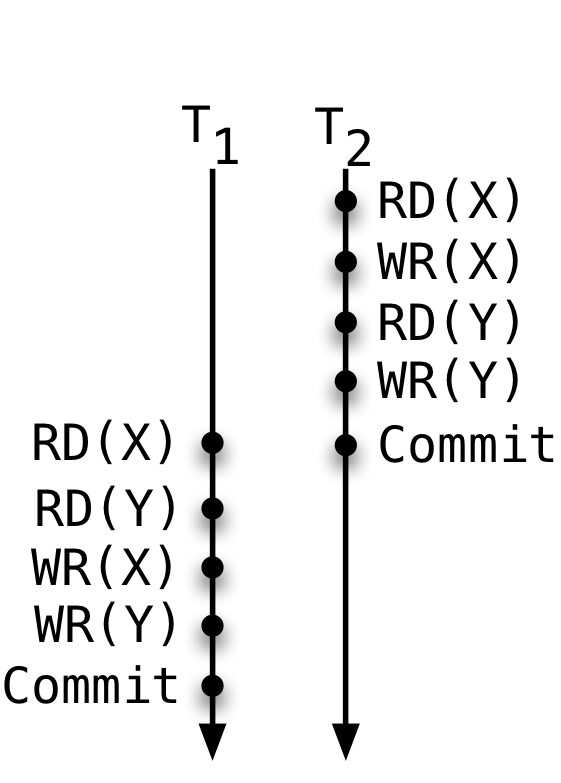
\includegraphics[scale=0.36]{Figures/rr-eg}
}
\subcaptionbox {
  {\sc si}($T_1$), {\sc mav}($T_2$)
  \label{fig:ansi-iso-eg-si}
} [
  0.33\columnwidth
] {
  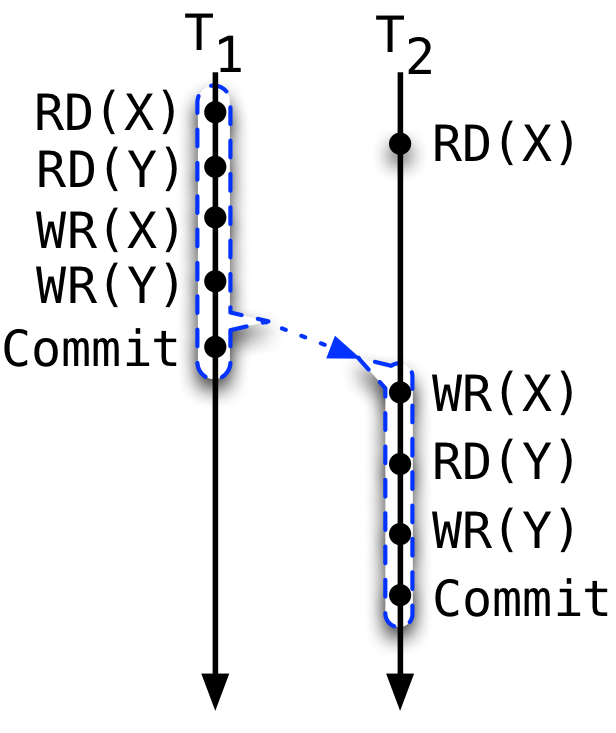
\includegraphics[scale=0.36]{Figures/si-eg-2}
}
\subcaptionbox {
  {\sc ser}($T_3$), {\sc mav}($T_4$)
  \label{fig:ansi-iso-eg-ser}
}{
  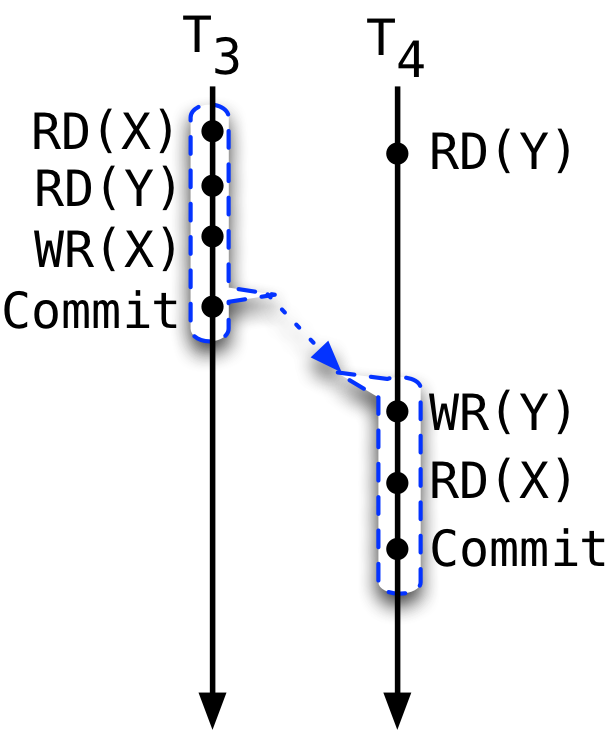
\includegraphics[scale=0.32]{Figures/ser-eg}
}

\caption{\small Sample executions of concurrent transactions at different
isolation levels. Solid (black) arrows indicate the timeline. Points
on the timeline mark the time when an operation is executed. Dotted
(blue) arrows denote $\visZ$. }
\label{fig:ansi-iso-eg}
\vspace*{-12pt}
\end{figure}

% Note that both $\mathtt{SnapshotVis}$ and $\mathtt{OneWaySER}$
% are asymmetric definitions that guarantee complete visiblity or
% invisibility of $T_i$ to $T_j$, but not the converse. While
% $\mathtt{SnapshotVis}$ provides no guarantees to $T_i$,
% $\mathtt{OneWaySER}$ guarantees that at least the commit effect of
% $T_i$ witnesses $T_j$. 

% \iso{Snapshot Isolation} spec ({\sc si}) extends {\sc rr} with a
% one-way serializability guarantee w.r.t. the transactions that perform
% conflicting writes (i.e., writes to the same shared variable).
% \footnote{Fig.~\ref{fig:ansi-isolation} presents slightly
% weaker versions of {\sc si} and {\sc ser} specs in the interest of
% clarity.}. Fig.~\ref{fig:ansi-iso-eg} shows sample executions of
% transactions $T_1$ and $T_2$. Both transactions read and write to
% shared variables $X$ and $Y$. In the first execution, $T_2$ commits
% while $T_1$ is still in progress, but {\sc rr} isolation prevents
% $T_1$ from witnessing the writes of $T_2$. In the second execution,

%% SJ: Not sure this paragraph is necessary here.
%% In contrast to recent proposals (\emph{e.g.},
%% ~\cite{gotsmanconcur15}), our specifications for {\sc si} and {\sc
%%   ser} do not necessarily impose a total order among transactions
%% (conflicting or otherwise). In reality, a total order under {\sc ser}
%% (resp. {\sc si}) is guaranteed only if the store executes all
%% transactions under {\sc ser} (resp. {\sc si}) isolation. Our
%% specifications admit this possibility, and derive a total order under
%% the assumption of homogenity. However, databases almost always allow
%% isolation levels to be configured on a per-transaction basis, allowing
%% transactions at various isolation levels to coexist.  Specifications
%% that assume homogenity are incorrect under this setting.

% Having specified isolation levels as trace well-formedness
% constraints, we can now construct trace invariants ($\I$) for
% \txnimp programs by composing isolation specifications for various
% transactions. For instance, the following trace invariant enforces
% {\sc si} for both transactions of the program in
% Fig.~\ref{fig:motiv-eg-1}, allowing it to satisfy its postcondition:
% \begin{smathpar}
% \I \;=\; \lambda\E.~ \underE{\C{SI(Wd1)}} \conj \underE{\C{SI(Wd2)}}
% \end{smathpar}
% In contrast, the following trace invariant enforces {\sc rc} for one and {\sc si}
% for another, leading to a possible violation of the postcondition:
% \begin{smathpar}
% \I \;=\; \lambda\E.~ \underE{\C{RC(Wd1)}} \conj \underE{\C{SI(Wd2)}}
% \end{smathpar}




\section{The Reasoning Framework}
\label{sec:reasoning}

We now describe a proof system that lets us prove the correctness of a \txnimp
program $c$ w.r.t its high-level invariant $I$, on a machine that
satisfies the isolation specifications ($\I$) of its
transactions\footnote{Note the difference between $I$ and $\I$. The
former constitute \emph{proof} \emph{obligations} for the programmer,
whereas the latter describes a transaction's \emph{assumptions} about
operational characteristics of the underlying machine.}.  Our proof
system is essentially an adapatation of the rely-guarantee reasoning
framework to the setting of weakly isolated database transactions. It
deals with the additional complexity introduced by this setting, while
also taking advantage of the opportunities it provides to simplify the
reasoning. The primary challenge is the weak isolation; how do we
relate a transaction's isolation specification ($\I$) to its rely
relation ($R$) that describes the environment, so that the
interference is considered only insofar as the isolation level allows
it? Our proof system shows how to compute a rely relation ($R$) modulo
the isolation specification ($\I$) of a transaction. Another
characteristic of the transaction setting is the atomicity of a
trasaction's aggregate writes; a transaction's writes are not visible
to its peers until it commits. In the context of rely-guarantee, this
means that the transactions guarantee ($G$) should capture the
aggregate effect of a transaction, and not its individual writes.
While \C{atomic} blocks are also present in the shared-memory
programs, the fact that a transactions are weakly isolated introduces
complexity.  Unlike an \C{atomic} block, the effect of a transaction
is \emph{not} a sequential composition of the effects of its
statements because each statement witnesses a potentially different
version of the state. This is illustrated in
Fig.~\ref{fig:atomic-vs-transaction}, where a series of operations on
\C{x} can be composed to describe the effect of an \C{atomic} block,
while same cannot be done in a transaction. Thus, weak isolation needs
to be taken into account when defining and verifying guarantees, and
our proof system shows how. 

\subsection{The Rely-Guarantee Judgment}
\label{sec:rely-guarantee}

\begin{figure}[t]
\raggedright
%
\fbox {\( \R \vdash \hoare{P}{c}{Q} \)} 
\quad \fbox {\( \rg{I,R}{c}{G,I} \)}\\[4pt]
%\fbox{\( \rg{\mathbb{I},P,R}{\txnbox{c}_i}{G,Q}\)} \quad
%\fbox{\( \rg{\mathbb{I},P,R}{c}{G,Q}\)} \quad\\
%
\begin{minipage}{3.1in}
\rulelabel{RG-Update}
\begin{smathpar}
\begin{array}{c}
\RULE
{
  \stable(\R,Q)\\
  \forall\stl,\stl',\stg.~P(\stl,\stg) \conj \\
  \stl' = \stl \cup \{r' \,|\, \exists(r\in\Delta).[r/x]e_2 \conj\\
  \hspace*{.7in} r'=[r/x]e_1\} \Rightarrow   Q(\stl',\stg)
}
{
  \R \vdash \hoare{P}{\updatee{\lambda x.e_1}{\lambda x.e_2}}{Q}
}
\end{array}
\end{smathpar}
\end{minipage}
%
%
\begin{minipage}{3in}
\rulelabel{RG-Select}
\begin{smathpar}
\begin{array}{c}
\RULE
{
  \\
  \R \vdash \hoare{P'}{c}{Q}\spc
  \stable(\R,P')\\
  P'(\stl,\stg) \Leftrightarrow P(\stl,\stg) \wedge
  x = \{r' \,|\, \exists(r\in\Delta).~ [r/y]e_2\} \\
}
{
  \R \vdash \hoare{P}{\lete{x}{\selecte{\lambda y.e}}{c}}{Q}
}
\end{array}
\end{smathpar}
\end{minipage}
%
\bigskip

%
\begin{minipage}{3.2in}
\rulelabel{RG-Delete}
\begin{smathpar}
\begin{array}{c}
\RULE
{
  \stable(\R,Q)\\
  \forall\stl,\stl',\stg.~P(\stl,\stg) \conj 
  \stl' = \stl \cup \{r' \,|\, \exists(r\in\Delta).~ [r/x]e
        \conj r'=\{\bar{f}=r.\bar{f}; \idf=r.\idf;
        \delf=\C{true}\}\}
  \Rightarrow 
  Q(\stl',\stg)
}
{
  \R \vdash \hoare{P}{\deletee{\lambda x.e}}{Q}
}
\end{array}
\end{smathpar}
\end{minipage}
%
\bigskip

%
\begin{minipage}{3.2in}
\rulelabel{RG-Insert}
\begin{smathpar}
\begin{array}{c}
\RULE
{
  \stable(\R,Q)\\
  \hspace*{-1.1in}\forall\stl,\stl',\stg,i.~P(\stl,\stg) \conj i \not\in
  \dom(\stl\cup\stg) \\
  \conj \stl'=\stl \cup 
  \{\{\bar{f}=x.\bar{f};\,\idf=i;\,\delf=\C{false}\} \Rightarrow 
  Q(\stl',\stg)
}
{
  \R \vdash \hoare{P}{\inserte{x}}{Q}
}
\end{array}
\end{smathpar}
\end{minipage}
%
%
\begin{minipage}{3in}
\rulelabel{RG-Foreach}
\begin{smathpar}
\begin{array}{c}
\RULE
{
  \stable(\R,Q)\spc
  \stable(\R,\psi)\\
  P \wedge y=\emptyset \Rightarrow \psi\spc
  \R \vdash \hoare{\psi \wedge z\in x}{c}{Q_c}\\
  Q_c \wedge z\in y \Rightarrow \psi\spc
  \psi \wedge y=x \Rightarrow Q
}
{
  \R \vdash \hoare{P}{\foreache{x}{\lambda y.\lambda z.c}}{Q}
}
\end{array}
\end{smathpar}
\end{minipage}
%
\bigskip

%
\begin{minipage}{3.9in}
\rulelabel{RG-Txn}
\begin{smathpar}
\begin{array}{c}
\RULE
{
  \stable(R,\I)\spc
  P(\stl,\stg) \Leftrightarrow \stl=\emptyset \wedge I(\stg)\\
  \R_l(\stl,\stg,\stg') \Leftrightarrow \exists \stg_1. \I_e(\stl, \stg_1, \stg) \wedge R(\stg, \stg') \wedge \I_e(\stl, \stg_1, \stg')\\
  \R_c(\stl,\stg,\stg') \Leftrightarrow \exists \stg_1. \I_c(\stl, \stg_1, \stg) \wedge R(\stg, \stg') \wedge \I_c(\stl, \stg_1, \stg')\\
  \R_l \vdash \rg{P}{c}{Q} \spc \stable(\R_c,Q)\\
  \forall \stl,\stg.~ Q(\stl,\stg) \Rightarrow 
    G(\stg, \stl \gg \stg)\spc
  \forall \stg,\stg'.~I(\stg) \wedge G(\stg,\stg') \Rightarrow I(\stg')\\
}
{
  \rg{I,R}{\ctxn{i}{\I}{c}}{G,I}
}
\end{array}
\end{smathpar}
\end{minipage}
%
%
\begin{minipage}{2in}
\rulelabel{RG-Conseq}
\begin{smathpar}
\begin{array}{c}
\RULE
{
  \rg{I,R}{\ctxn{i}{\I}{c}}{G,I}\\
  \I' \Rightarrow \I \spc 
  R' \subseteq R \\
  \stable(R',\I')\spc
  G \subseteq G' \\
  \forall \stg,\stg'.~I(\stg) \wedge G'(\stg,\stg') \Rightarrow I(\stg')\\
}
{
  \rg{I,R'}{\ctxn{i}{\I'}{c}}{G',I}
}
\end{array}
\end{smathpar}
\end{minipage}
%

\caption{\small \txnimp: Rely-Guarantee Rules}
\label{fig:rg-rules}
\vspace*{-12pt}
\end{figure}


Fig.~\ref{fig:rg-rules} shows an illustrative subset of the
rely-guarantee (RG) reasoning rules for $\txnimp$. We define two RG
judgments: top-level ($\rg{I,R}c{G,I}$), and transaction-local ($\R
\vdash \hoare{P}c{Q}$).  Recall that the standard RG judgment is the
quintuple $\rg{P,R}{c}{G,Q}$. Instead of a separate $P$ and $Q$, our
top-level judgment has $I$ for both pre- and post-conditions, because
our focus is on verifying that a \txnimp program \emph{preserves}
database's consistency conditions\footnote{The terms \emph{consistency
condition}, \emph{high-level invaraint}, and \emph{integrity
constraint} all mean the same.}. Transaction-local RG judgment doesn't
include a guarantee relation because transaction-local effects are not
visible outside a transaction. Also, the rely relation ($\R$) of the
transaction-local judgment is not same as the top-level rely relation
($R$) as it takes into account the transaction's isolation
specification ($\I$). Intuitively, $\R$ is $R$ modulo $\I$; formal
definition will be given shortly. Recall that a transaction writes to
its local database ($\stl$), which is then flushed when the
transaction commits. Thus, the guarantee of a transaction depends on
the state of its local database at the commit point. The pre- and
post-condition assertions ($P$ and $Q$) in the local judgment
facilitate tracking the changes to the transaction-local state, which
eventually helps us prove the validity of the transaction's guarantee.
Note that $P$ and $Q$ are bi-state assertions; they relate
transaction-local database state ($\stl$) to the global database state
($\stg$). Thus, the transaction-local judgment effectively tracks how
transaction-local and global states change in relation to each other.

The quintessential aspect of a rely-guarantee judgment is the
stability condition, which, intuitively, requires the validity of an
assertion $\phi$ to be unaffacted by the interference, i.e., the rely
relation $R$. In conventional RG, stability is defined as following
($\sigma$ denotes a state):
\begin{smathpar}
\begin{array}{lcl}
\stable(R,\phi) & \Leftrightarrow & \forall \sigma,\sigma'.~
\phi(\sigma) \conj R(\sigma,\sigma') \Rightarrow \phi(\sigma')\\
\end{array}
\end{smathpar}
Due to the presence of local and global database states, and isolation
specification, we use multiple definitions of stability in
Fig.~\ref{fig:rg-rules}, but they all convey the same intuition as
above. We will introduce them as they are encountered.

\rulelabel{RG-Txn} is the top-level rule that lets us prove a
transaction preserves the high-level invariant $I$ when executed under
the required isolation as specified by $\I$. It relies on the
transaction-local judgment to verify the the transaction body ($c$).
The precondition $P$ of $c$ must follow from the fact that the
transaction-local database ($\stl$) is initially empty, and the global
database satisfies the high-level invariant $I$. The rely relation
($\R_l$) for the local judgment is a ternary relation computed as $R$
modulo $\I$ as following:
\begin{smathpar}
\begin{array}{lcl}
\R_l(\stl,\stg,\stg') & \Leftrightarrow & R(\stg,\stg') \conj
\I\,\C{true}\,(\stl,\stg,\stg')
\end{array}
\end{smathpar}
Thus, $\R_l$ allows an interference only if it doesn't violate the
execution-time isolation specification of the transaction. If a
certain interference violates the isolation spec, i.e., $R(\stg,\stg')
\Rightarrow \neg(\I\,\C{true}\,(\stl,\stg,\stg'))$, then
$\R_l(\stl,\stg,\stg') \Leftrightarrow false$, and any assertion is
trivially stable w.r.t that interference. This is sensible considering
such interference is pre-empted in the operational semantics. 

Recall that $P$ and $Q$ of the transaction-local RG judgment are
binary assertions; they relate local and global database states. The
local judgment rules require one or both of them to be stable. The
stability of a binary assertion $Q$ w.r.t a ternary rely relation $\R$
is defined as following:
\begin{smathpar}
\begin{array}{c}
\forall \stl,\stg,\stg'.~ Q(\stl,\stg) \conj \R(\stl,\stg,\stg')
\Rightarrow Q(\stl,\stg')
\end{array}
\end{smathpar}
That is, if $Q$ relates $\stl$ to $\stg$, and an interference allowed
by the isolation specfication (which implicitly considers the local
state $\stl$) takes $\stg$ to $\stg'$, the $Q$ must also relate $\stl$
to $\stg'$.

For the guarantee $G$ of the transaction to be valid, it must follow
from the post-condition $Q$ of the body, provided that $Q$ is stable
w.r.t the commit-time interference captured by $R_c$. $R_c$, like
$R_l$, is computed as rely relation modulo isolation, except that
commit-time isolation ($\I\,\C{false}$) is considered. The validity of
$G$ is captured by the following implication:
\begin{smathpar}
\begin{array}{c}
  \forall \stl,\stg.~ Q(\stl,\stg) \Rightarrow G(\stg, \stl \gg \stg)\spc
\end{array}
\end{smathpar}
In other words, if $Q$ relates the transaction-local database state
($\stl$) to the state of the global database ($\stg$) before the
commit, then $G$ must relate the states of the global database before
and after the commit. The act of commit captured by the flush
operation ($\stl\gg\stg$). Once we establish the validity of $G$ as a
faithful representative of the transaction, we can verify that the
transaction preserves the high-level invariant $I$ by checking the
stability of $I$ w.r.t $G$, i.e., $\forall \stg,\stg'.~I(\stg) \wedge
G(\stg,\stg') \Rightarrow I(\stg')$.

A characteristic of RG reasoning is that stability of an assertion is
always proven w.r.t to $R$, and not $R^{*}$, although interference may
include multiple environment steps, and $R$ only captures a single
step. This is nonetheless sound due to the the inductive reasoning: if
$Q$ is preserved by every step of $R$, then $Q$ is preserved by
$R^{*}$, and vice-versa.  However, such reasoning does not extend
naturally to isolation-constrained interference because $R^{*}$ modulo
$\I$ is not same as $\R^{*}$; the former is a transitive relation
constrained by $\I$, whereas the latter is the transitive closure of a
$\I$-constrained relation. We therefore introduce a side-condition on
$\I$ that restores the equality. The condition requires $\I$ to allow
an intereference $R^{*}(\stg,\stg'')$, for two database states $\stg$
and $\stg''$, only if it also allows interference for every prefix of
$R^{*}(\stg,\stg'')$. In other words, if $\I$ disallows interference
from $\stg$ to $\stg'$, then an $R$-step from $\stg'$ to $\stg''$
shouldn't make the interference from $\stg$ to $\stg''$ valid. We call
this the stability condition on $\I$, defined as below:
\begin{smathpar}
\begin{array}{lcl}
  \stable(R,\I) & \Leftrightarrow & \forall \stl,\stg,\stg',\stg''.~
  \neg\I(\stl,\stg,\stg') \conj R(\stg',\stg'') \Rightarrow
  \neg\I(\stl,\stg,\stg'')
\end{array}
\end{smathpar}
It can be easily verified that the above stability condition is
satisfied by the isolation axioms from Sec.~\ref{sec:isolation}. For
instance, $\I_{ss}$, the snapshot axiom, is stable because if
$\I_{ss}$ is invalid, then an interference has already modified a
record, and no further interference will restore the original record,
because original record bears the id of a transaction that has long
committed. Thus, $\I_{ss}$ remains invalid.

The \rulelabel{RG-Conseq} rule lets us safely strengthen the guarantee
$G$, or weaken the rely $R$ of a transaction. Importantly, it also
allows its isolation specification $\I$ to be strengthened. This means
that a transaction proven correct under a weaker isolation level is
also correct under a stronger level. Parametricity over the isolation
specification $\I$, combined with the ability to strengthen $\I$ as
needed, admits a flexible proof strategy to prove database programs
correct. For example, programmers can declare isolation requirements
of their choice through $\I$, and then prove programs correct assuming
the guarantees hold. The soundness of strengthening $\I$ ensures that
a program can be safely executed on any system that offers isolation
guarantees at least as strong as those assumed.

Two rules of the transaction-local RG judgment are shown in
Fig.~\ref{fig:rg-rules}. The rule \rulelabel{RG-Update} is
illustrative of the RG rules for SQL statements; they basically
reflect the structure of the corresponding reduction rule from
Fig.~\ref{fig:txnimp}, and require no further explanation. The rule
\rulelabel{RG-Foreach} defines the RG judgment for a \C{FOREACH} loop.
As is characteristic of loops, the reasoning is pivoted on a loop
invariant $\I$ (not same as the high-level invariant), that needs to
be stable w.r.t $\R$. $I$ must follow $P$, the pre-condition of
\C{FOREACH}, when no elements have been iterated, i.e, when
$y=\emptyset$. The body of the loop can assume the loop invariant, and
the fact that $z$ is an element from the set $x$ being iterated, to
prove its post-condition $Q_c$. Operational semantics ensures that $z$
is added to $y$ at the end of the iteration, hence $Q_c \conj z\in y$
is valid at the end of the iteration, from which $I$ must follow. When
\C{FOREACH} has finished execution, $y$, the set of iterated items, is
the entire set $x$. Thus $I \conj y=x$ must imply the post-condition
$Q$, which also needs to be stable. The rules for conditions,
sequencing etc., are more-or-less standard, hence elided.

% \subsection{Semantics and Soundness}

% The rules that define rely-guarantee judgment are shown in
% Fig.~\ref{fig:rg-rules}. Like standard rely-guarantee definitions,
% these definitions also require a \emph{stability} condition, which
% requires pre- and post- conditions to hold despite any interference
% from concurrent threads (captured by $R$). Stability can be predicated
% on the assumption that interference preserves the trace invariant
% $\I$. Formally:\vspace*{-10pt}

% \begin{smathpar}
% \begin{array}{lcl}
%   \underI{\stable(R,P)} & \defeq & \forall \E, \E'.\, 
%   \I(\E) \conj P(\E) \conj R(\E,\E') \\
%   &   & \hspace*{1in}\conj \I(\E') \Rightarrow P(\E')\\
% \end{array}
% \end{smathpar}

% \noindent However, the assumption that interference preserves $\I$ (or,
% dually, $\I$ withstands interference) needs to be justified
% separately. We call this the stability requirement on $\I$:\vspace*{-10pt}

% \begin{smathpar}
% \begin{array}{lcl}
% \stable(R,\I)& \defeq & \forall \E, \E'.\, 
%   \I(\E) \conj R(\E,\E')\Rightarrow \I(\E')\\
% \end{array}
% \end{smathpar}

% \noindent The rule \rulelabel{RG-Var} defines the rely-guarantee judgment for
% shared variable reads inside a transaction $T_i$. It requires $\I$ to
% be stable, and pre- and post- conditions to be stable relative to
% $\I$.  The quantified premise effectively requires a proof that if the
% abstract machine of Fig.~\ref{fig:txnimp} takes a step starting from
% an execution $\E$ that satisfies the pre-condition $P$, then the
% resultant execution $\E'$ satisfies the post-condition $Q$, and that
% the guarantee $G$ faithfully captures the transition from $\E$ to
% $\E'$. It is informative to compare this premise with the premise of
% the \rulelabel{E-Aux} reduction rule of Fig.~\ref{fig:txnimp}. Similar
% premises also appear in the \rulelabel{RG-Asgn} and \rulelabel{RG-Txn}
% rules, which define rely-guarantee judgments for assignments and
% transactions, respectively. \rulelabel{RG-Var} however also requires
% the return value ($\interp{S}(X)$) of the read to satisfy the
% assertion $C$ meant for the value. \rulelabel{RG-Arith} defines the RG
% judgment for an arithmetic expression $e_1\pm e_2$ in terms of the
% corresponding judgments for the constituent expressions $e_1$ and
% $e_2$. The quantified premise requires any value resulting from
% evaluating $e_1 \pm e_2$ to satisfy the assertion $C$, provided that
% $e_1$ and $e_2$ always evaluate to values that satisfy $C_1$ and
% $C_2$, respectively. The rules for sequential and parallel composition
% of commands are essentially the same as their counterparts in a
% standard rely-guarantee formulation and hence elided.

% % RG judgment for the assignment $X:=e$ makes use of the corresponding
% % judgment for the RHS expression $e$. The quantified premise asserts
% % that evaluating the assigment after evaluating $e$ to a value $v$ and
% % an execution $\E$, should result in an execution $\E'$ that satisfies
% % the post-condition $Q$, while being related to $\E$ via the guarantee
% % $G$. RG judgment for the \C{txn} lexical block is similar.  It uses
% % the judgment for the transaction-bound command $c$ (i.e.,
% % $\txnbox{c}_i$) to obtain an invariant $Q'$ for the execution $\E$
% % before the commit, and verifies that committing the transaction under
% % $\E$ results in an execution $\E'$ that satisfies transaction's
% % post-condition $Q$. As usual, $\E$ and $\E'$ need to be related by $G$.
% % The rules for sequential composition of transaction-bound comands
% % (\rulelabel{RG-Seq}) and parallel composition of top-level commands
% % (\rulelabel{RG-Par}) are straightforward, and more-or-less same as the
% % corresponding rules in classical rely-guarantee.

% The \rulelabel{RG-Conseq} rule defines ways to strengthen or
% weaken relations and assertions associated with the RG judgment of
% transaction-bound expressions. Similar rules exist for
% transaction-bound and top-level commands, but are not
% shown.\footnote{The supplementary materials provide the complete set
%   of rules.} As is the case with a standard rely-guarantee
% formulation,the rules allow the pre-condition $P$ and the rely relation
% $R$ to be strengthened, and the post-condition $Q$ (also, $C$ in the
% case of expressions) and the guarantee relation $G$ to be weakened.
% The most notable aspect of the \rulelabel{RG-Conseq} rules is that
% they allow the trace invariant $\I$ to be strengthened. Considering
% that $\I$ captures isolation properties, this means that a program
% proven correct under weaker isolation levels is also correct under
% stronger ones.  Parametricity over the trace invariant $\I$, combined
% with the ability to strengthen $\I$ as needed, allows our proof system
% to support a highly flexible proof strategy to prove programs correct
% over various isolation variants. For example, programmers can
% \emph{define} isolation guarantees of their choice (by defining $\I$
% appropriately) and then prove programs correct assuming the guarantees
% hold.  The soundness of strengthening $\I$ ensures that a program can
% be safely executed on any system that offers isolation guarantees
% at least as strong as those assumed.

\subsection{Semantics and Soundness}

\begin{definition}[\bfseries Step-indexed reflexive transitive closure]
For all $A:\text{Type}$, $R: A \rightarrow A \rightarrow \mathbb{P}$, and $n :
\mathbb{N}$, the step-indexed reflexive transitive closure $R^n$ of $R$ is
the smallest relation satisfying the following
properties:
\begin{itemize}
\item $\forall (x:A).\, R^0 (x,x)$
\item $\forall (n:\mathbb{N})(x,y,z : A).\, R(x,y) \conj R^n(y,z) \Rightarrow
R^{n+1}(x,z)$
\end{itemize}
\end{definition}

\begin{definition}[\bfseries Interleaved step and multi-step relations]
An interleaved step relation interleaves thread-local reductions with
interference from concurrent threads captured as the rely relation
($R$).  It is defined thus:\vspace*{-10pt}

\begin{smathpar}
\begin{array}{lcl}
\I \vdash (c,\E) \rstepsto (c',\E') & \defeq & \I \vdash 
  (c,\E) \stepsto (c',\E') \\
  &   & \disj (c' = c \conj R(\E, \E') \conj \I(\E'))\\
\end{array}
\end{smathpar}

\noindent The interleaved step relation for transaction bound expressions
($\txnbox{e}_i$) and commands ($\txnbox{c}_i$) is defined similarly.
An interleaved multi-step relation ($\stepssto{n}$) is the step-indexed
reflexive transitive closure of the interleaved step relation.
\end{definition}

\begin{definition}[\bfseries Semantics of the RG judgment]
\label{def:rg-semantics}
The semantics of the RG sextuple $\rg{\mathbb{I},P,R}{c}{G,Q}$ is defined
in terms of the interleaved step relation thus:\vspace*{-10pt}

\begin{smathpar}
\begin{array}{l}
\hspace*{-0.3in}
\rg{\mathbb{I},P,R}{c}{G,Q} \;\defeq\; \forall \E.\, P(\E)
  \wedge \mathbb{I}(\E) \\
\hspace*{0.4in}\Rightarrow (\forall n,\E'.\; \I \vdash (c,\E) 
    \rstepssto{n} (\cskip,\E') \Rightarrow Q(\E')) \\
\hspace*{0.5in}\conj \texttt{step-guaranteed}(\I,R,G,c,\E)\\
\end{array}
\end{smathpar}

\noindent The first conjunct in the consequent is called the \emph{Hoare
consequent} since it ascribes Hoare triple semantics to an RG sextuple.
The second conjunct, called the \emph{guarantee consequent}, uses the
$\texttt{step-guaranteed}$ predicate defined below:\vspace*{-10pt}

\begin{smathpar}
\begin{array}{l}
\texttt{step-guaranteed}(\I,R,G,c,\E) \;\defeq\; \forall n,\E',c'',\E''.\\
\hspace*{0.2in}\I \vdash (c,\E) \rstepssto{n} (c',\E') \conj \I \vdash (c',\E') \stepsto
  (c'',\E'') \Rightarrow G(\E',\E'')\\
\end{array}
\end{smathpar}

\noindent The guarantee consequent requires $G$ to capture the trace effect of
every small-step of $c$, where the reduction can be interleaved by the
interference ($R$) from concurrent threads. The semantics of the RG
sextuple for transaction-bound commands ($\txnbox{c}_i$) is defined
similarly. Expressions, unlike commands, evaluate to a value $v$, and
the semantics of their RG septuple ($\rg{\I,P,R}{\txnbox{e}_i}{G,C,Q}$) differs slightly in that its
Hoare consequent requires the value $v$ to satisfy the assertion $C$. 
\end{definition}

Note that the semantics of all RG judgments, including the judgments
for transaction-bound terms, make similar demands of the guarantee
relation. Given that transactions are atomic (though not isolated), it
is not immediately apparent why a transaction's guarantee is required
to make explicit every step of its reduction. This requirement is
justified however because, in reality, a transaction's atomicity is
predicated on the isolation settings of the observer. A \iso{Read
  Uncommitted} transaction, for example, is permitted to observe the
internal state of a transaction $T$ even if $T$ is claimed to execute
atomically.  In the interest of modular verification, the transaction
must therefore make its internal state available via its guarantee
relation.

\begin{theorem}[\bfseries Soundness] 
The rely-guarantee judgments defined by the rules in
Fig.~\ref{fig:rg-rules} are sound with respect to the semantics of
Definition~\ref{def:rg-semantics}.\footnote{Formal proof of soundness
is provided in the supplementary material.}
\end{theorem}

\noindent In particular, if $\rg{\I,P,R}{c}{G,Q}$ can be derived using
the rules of Fig.~\ref{fig:rg-rules}, then (a) every interleaved
multi-step reduction of $c$ starting from a trace that satisfies $P$
and $\I$, results in a trace that satisfies $Q$, and (b) the effect
that every small-step of $c$ has on the trace is contained in $G$.
Soundness of the RG judgment for transaction-bound commands
($\txnbox{c}_i$) is stated similarly.  For expressions, soundness of
the judgment $\rg{\I,P,R}{\txnbox{e}_i}{G,C,Q}$ also proves that $e$
is always evaluated to a value that satisfies $C$.



\section{Inference}
\label{sec:inference}

The rely-guarantee framework presented in the previous section
facilitates modular proofs for weakly-isolated transactions, but
imposes a non-trivial annotation burden.  In particular, it requires
each statement ($c$) of the transaction to be annotated with a stable
pre- ($P$) and post-condition ($Q$), and loops to be annotated with
stable inductive invariants ($\psi$). While weakest pre-condition
style predicate transformers can help in inferring intermediate
assertions for regular statements, loop invariant inference remains
challenging, even for the simple form of loops considered here.  As an
alternative, we present an inference algorithm based on state
transformers that alleviates this burden.  The idea is to infer the
logical effect that each statement has on the transaction-local
database state $\stl$ (i.e., how it transforms $\stl$), and compose
multiple such effects together to describe the effect of the
transaction as a whole.  Importantly, this approach generalizes to
loops, where the effect of a loop can be inferred as a well-defined
function of the effect of its body, thanks to certain pleasant
properties enjoyed by the database programs modeled by our core
language.  Interpreting database semantics as functional
transformations on sets (described in terms of their logical effects)
enables an inference mechanism that can leverage off-the-shelf SMT
solvers for automated verification.

\begin{figure}[h]
\begin{smathpar}
\renewcommand{\arraystretch}{1.2}
\begin{array}{lcl}
\multicolumn{3}{c}{
  x,y,\stl,\stg \in \texttt{Variables}\spc
  \varphi \in \Prop^{0}\spc
  \phi \in \Prop^{1}
}\\
s & \coloneqq & x \ALT \stl \ALT \stg \ALT \{x \,|\, \varphi\} 
  \ALT \existsl(\stg,\phi,s) 
  \ALT s_1 \bind \lambda x. s_2 \ALT \itel{\varphi}{s_1}{s_2} 
  \ALT s_1 \cup s_2 \\
\end{array}
\end{smathpar}
%
\caption{Syntax of the set language $\SL$}
\label{fig:logic-syntax}
\end{figure}



At the core of our approach is a simple language ($\SL$) to express
set transformations (see Fig.~\ref{fig:logic-syntax}). The language
admits set expressions that include variables ($x$), literals of the
form $\{x \,|\, \varphi\}$ where $\varphi$ is a propositional
(quantifier-free) formula on $x$, a restricted form of existential
quantification that binds a set $\stg$ satisfying proposition $\phi$
in a set expression $s$, a monadic composition of two set expressions
($s_1$ and $s_2$) composed using a bind ($\bind$) operation, a
conditional set expression where the condition is a propositional
formula, and a union of two set expressions. Symbols $\stl$ and $\stg$
are also variables in $\SL$, but are used to denote local and database
states (also represented as sets), respectively. Constant sets can be
written using set literal expressions. For example, the set $\{1,2\}$
can be written as $\{x \,|\, x=1 \vee x=2\}$. The language is
carefully chosen to be expressive enough to capture the semantics of
$\txnimp$ statements (as well as SQL operations more generally), yet
simple enough to have a semantics-preserving translation amenable for
automated verification.

\begin{figure}
\raggedright
%
\fbox {\(c \elabsto \F \)}\\
%

% \renewcommand{\arraystretch}{1.2}
% \begin{smathpar}
% \begin{array}{lcl}
% % \inserte{x} & \elabsto & \stabilize{\lambda(\stl,\stg).~
% %   \{ r \,|\, r = \{x \with \idf = \uid(x);\,r.\delf=\C{false};\,
% %                 \txnf = i\} \conj \uid(x) \notin \dom(\stl\cup\stg) \}}\\ 
% %
% %
% \updatee{\lambda x.e_1}{\lambda x.e_2} & \elabsto & \stabilize{
%   \lambda(\stl,\stg).~ \stg \bind (\lambda r.~ 
%   \{r' \,|\, [r/x]e_2 \conj r' = \{[r/x]e_1 \with 
%       \idf=r.\idf;\,\delf = r.\delf;\,\txnf=i \}) \} }\\ 
% %
% \deletee{\lambda x.e} & \elabsto & \stabilize{
%   \lambda(\stl,\stg).~ \stg \bind (\lambda r.~ 
%   \{r' \,|\, [r/x]e \conj r'=\{r \with \delf=\C{true}\})\} }\\ 
% %
% \end{array}
% \end{smathpar}

\begin{center} 
%
%\begin{minipage}{3.5in}
\begin{smathpar}
\begin{array}{c}
\RULE
{
}
{
  \inserte{x} ~\elabsto~ \stabilize{\lambda(\stl,\stg).~
    \{ y \,|\, y = \{\langle x \with r.\delf=\mathtt{false};\, \txnf = i\rangle \}}
}
\end{array}
\end{smathpar}
%\end{minipage}
%\begin{minipage}{3.5in}
\begin{smathpar}
\begin{array}{c}
\RULE
{
  G = \lambda y.~ \itel{[y/x]e_2}
      {\{\langle[y/x]e_1 \with \idf=r.\idf;\,\delf = y.\delf;\,\txnf=i\rangle \}}
      {\emptyset}
}
{
  \updatee{\lambda x.e_1}{\lambda x.e_2}  ~\elabsto~
  \stabilize{\lambda(\stl,\stg).~ \stg \bind G } 
}
\end{array}
\end{smathpar}
%\end{minipage}
%\begin{minipage}{3in}
\begin{smathpar}
\begin{array}{c}
\RULE
{
  G = \lambda y.~ \itel{[y/x]e}
      {\{\langle y \with \delf = \mathtt{true};\,\txnf=i\rangle \}}
      {\emptyset}
}
{
  \deletee{\lambda x.e}  ~\elabsto~
  \stabilize{
  \lambda(\stl,\stg).~ \stg \bind G \} }
}
\end{array}
\end{smathpar}
%\end{minipage}

%\begin{minipage}{2.7in}
\begin{smathpar}
\begin{array}{c}
\RULE
{
  c \elabsto \F \spc
}
{
  \lete{x}{e}{c} ~\elabsto~  
    \stabilize{\lambda(\stl,\stg).~ [e/x]\,\F(\stl,\stg)}\\
}
\end{array}
\end{smathpar}
%\end{minipage}

%\begin{minipage}{3in}
\begin{smathpar}
\begin{array}{c}
\RULE
{
  c \elabsto \F \spc
  G = \lambda r.~ \itel{[r/x]e}{\{x\ |\ x = r \}}{\emptyset}
}
{
  \lete{y}{\selecte{\lambda x.e}}{c} ~\elabsto~  
    \stabilize{\lambda (\stl,\stg).~ [(\stg \bind G)/y]\,\F(\stl,\stg)}\\
}
\end{array}
\end{smathpar}
%\end{minipage}

%\begin{minipage}{3.2in}
\begin{smathpar}
\begin{array}{c}
\RULE
{
  c_1 \elabsto \F_1 \spc
  c_2 \elabsto \F_2 
}
{
  \ite{e}{c_1}{c_2} ~\elabsto~
    \lambda(\stl,\stg).~\itel{e}{\F_1(\stl,\stg)}{\F_2(\stl,\stg)}\\
}
\end{array}
\end{smathpar}
%\end{minipage}

%\begin{minipage}{3in}
\begin{smathpar}
\begin{array}{c}
\RULE
{
  c_1 \elabsto \F_1 \spc
  c_2 \elabsto \F_2 
}
{
  c_1;c_2 ~\elabsto~  \lambda(\stl,\stg).~\F_1(\stl,\stg) \cup \F_2(\stl \cup \F_1(\stl,\stg),\stg)
}
\end{array}
\end{smathpar}
%\end{minipage}
%

%
%\begin{minipage}{3in}
\begin{smathpar}
\begin{array}{c}
\RULE
{
  c \elabsto \F \spc
}
{
  \foreache{x}{\lambda y.\lambda z.~c} ~\elabsto~
  \lambda(\stl,\stg).~ x\bind(\lambda z.~\F(\stl,\stg))
}
\end{array}
\end{smathpar}
%\end{minipage}

\end{center}
%

\caption{\txnimp: State transformer semantics. }
\label{fig:inference-rules}
\end{figure}


Fig.~\ref{fig:inference-rules} shows the syntax-directed state
transformer inference rules for $\txnimp$ commands inside a
transaction $\C{TXN}_i$. The rules compute, for each command $c$, a
(meta) function $\F$ that returns a set of records as an expression in
$\SL$, given a global database $\stg$. Intuitively, $\F(\stg)$
abstracts the set of records added to the local database $\stl$ as a
result of executing $c$ under $\stg$ (i.e., $\stg \vdash
(\tbox{c}_i,\stl) \stepsto^{*}_{R} (\tbox{\cskip}_i, \stl \cup
\F(\stg))$)\footnote{Recall that the operational semantics treats 
  deletion of records as the addition of the deleted record with its
  \C{del} field set to true in the local store.}. Note that the
  function $\F$ we call state transformer here is actually the
  \emph{effect} part of the state transformer introduced in
  Sec.~\ref{sec:motivation}, which is a function $\T$ of form
  $\lambda(\stl,\stg).~\stl \cup \F(\stg)$. Nonetheless, for
  simplicity, we will continue to refer to $\F$ as state transformer.
  Since the execution is subject to isolation-constrained
  interference, the inference judgment depends on the
  isolation-constrained rely relation $\R$, which is used to enforce
  the stability of the state transformer $\F$.  Recall that $\R$ is a
  tri-state rely relation over $\stl$, $\stg$ and $\stg'$, that admits
  an interference from $\stg$ and $\stg'$ depending on the local
  database state $\stl$. Thus, the stability of the state transformer
  $\F$ of $c$ with respect to $\R$ needs to take into account the
  (possible) prior state of the local database $\stl$, which depends
  on the context (sequence of previous commands) of $c$, and computed
  by the corresponding state transformer $\Fx$. Thus, the semantics of
  the state transformer can be understood in terms of the RG judgment
  as following (formalized as Theorem~\ref{thm:inference-sound} in
  Sec.~\ref{sec:inference-sound}):
\begin{smathpar}
  \begin{array}{c}
    \R \vdash \hoare{\lambda(\stl,\stg).~ \stl = \Fx(\stg)}{c}
    {\lambda(\stl,\stg).~ \stl = \Fx(\stg) \cup \F(\stg)}
  \end{array}
\end{smathpar}
In the above RG judgment, let $P$ denote the pre-condition
$\lambda(\stl,\stg).~ \stl = \Fx(\stg)$, and let $Q$ denote the
post-condition $\lambda(\stl,\stg).~ \stl = \Fx(\stg) \cup \F(\stg)$.
The stability condition on the state transformer $\F$ can be derived
from the stability condition on $Q$. Observe that for $Q$ to be
stable, $\Fx(\stg') \cup \F(\stg')$ must be equal to $\Fx(\stg) \cup
\F(\stg)$, where $\stg$ and $\stg'$ are related by $R$ (ignore $\I$
for the moment). Assuming that $P$ is stable, $\Fx(\stg')=\Fx(\stg)$
is already given, leaving $\F(\stg')=\F(\stg)$ to be enforced. Thus,
the stability of $\F$ in in the context of $\Fx$ (written
$\inctxt{\Fx}{\F}$) is defined as following:
\begin{smathpar}
\begin{array}{lcl}
  \stable(\R,\inctxt{\Fx}{\F}) & \Leftrightarrow & \forall \stg,\stg',\nubar.~
  \R(\Fx(\stg) \cup \F(\stg),\stg,\stg') \Rightarrow \F(\stg) = \F(\stg')
\end{array}
\end{smathpar}
where $\nubar$ are the variables that occur free in $\F$; this is
possible because of how the inference rules are structured. The
equality in $\SL$ translates to equivalence in first-order logic, as
we describe later. In the inference rules, stability is enforced
constructively by a meta-function $\stabilize{\cdot}$, which accepts
a transformer $\F$ (in its context $\Fx$) and returns a new
transformer that is guaranteed to be stable under $\R$.
$\stabilize{\cdot}$ achieves the stability guarantee by abstracting
away the bound global state ($\stg$) in an unstable $\F$ to an
existentially bound $\stg'$ as described below:
\begin{smathpar}
\begin{array}{lcll}
  \stabilize{\inctxt{\Fx}{\F}} & = & \F & \texttt{if }
  \stable(\R,\inctxt{\Fx}{\F}).\\
  & = & \lambda (\stg).~\existsl(\stg',I(\stg'),\F(\stg')) 
      & \texttt{otherwise. }\stg'\texttt{ is a fresh name.}\\
\end{array}
\end{smathpar}
Observe that when $\F$ is not stable, $\stabilize{\F}$ returns a
transformer $\F'$ that simply ignores its $\stg$ argument in favor of
a generic $\stg'$, making $\F'$ trivially stable. It is safe to assume
$I(\stg')$ because all verified transactions must preserve the
invariant, and hence only valid database states will ever be
witnessed. From the perspective of RG reasoning, $\stabilize{\cdot}$
effectively weakens the post-condition of a statement, as done by the
\rulelabel{RG-Conseq} rule for transaction-bound commands.  The
weakening semantics chosen by $\stabilize{\cdot}$, while being simple,
is nonetheless useful because of the $I(\stg')$ assumption imposed on
an existentially bound $\stg'$. The example in
Fig.~\ref{fig:weakening-example} demonstrates.
\begin{figure}[h]
\begin{center}
\begin{ocaml}
let add_interest acc_id pc = atomically_do @@ fun () ->
  let a = SQL.select1 BankAccount (fun acc -> acc.id = acc_id) in
  let y = a.bal + pc*a.bal in
  SQL.update BankAccount (fun acc -> {acc with bal = acc.bal + y})
                         (fun acc -> acc.id = acc_id)
\end{ocaml}
\end{center}
\caption{A transaction that deposits an interest to a bank account.}
\label{fig:weakening-example}
\end{figure}
Here, an \C{add\_interest} transaction adds a positive interest
(determined by \C{pc}) to the balance of a bank account, which is
required to be non-negative ($I(\stg) \Leftrightarrow
\forall(r\in\stg).~r.\C{bal}\ge 0$). The transaction starts by issuing
a \C{select1} query, whose transformer $\F$ is essentially a singleton
set containing a record $r$ whose id is \C{acc\_id} (i.e.,
$\F(\stg) = \{r \,|\, r\in\stg \wedge r.\C{id} = \C{acc\_id}\}$).
However, $\F$ is unstable because $\F(\stg')$ may not be
the same set as $\F(\stg)$ when $\stg'\neq\stg$. A record
$r\in\stg$ whose $\C{id}=\C{acc\_id}$ may have its balance updated by
a concurrent \C{withdraw} or \C{deposit} transaction in $\stg'$,
making the record in $\stg'$ different from the record in $\stg$.
Hence the stability check fails.  Fortunately, the weakening operator
($\stabilize{\cdot}$) allows us to weaken the effect to
$\existsl(\stg, I(\stg), \{ r \,|\, r\in\stg \wedge
r.\C{id}=\C{acc\_id}\})$, which effectively asserts that the
\C{select1} query returns a record with $\C{id}=\C{acc\_id}$ from
\emph{some} database state that satisfies the non-negative balance
invariant $I$.  This weakened assertion is nonetheless enough to
deduce that $\C{a.bal}\ge0$, and subsequently prove that $\C{a.bal +
pc*a.bal}\ge 0$, allowing us to verify the \C{add\_interest}
transaction.

The state transformer rules, like the earlier RG rules, closely follow
the corresponding reduction rules in Fig.~\ref{fig:txnimp}, except
that their language of expression is $\SL$. For instance, while the
reduction rule for \C{UPDATE} declaratively specifies the set of
updated records, the state transformer rule uses $\SL$'s bind
operation to \emph{compute} the set. Other SQL rules do likewise. The
rules for \C{LET} binders, conditionals, and sequences compose the
effects inferred for their subcommands. Thus, the effect of a sequence
of commands $c_1;c_2$ is the union of effects $\F_1$ and $\F_2$ of
$c_1$ and $c_2$, respectively, except that $\F_2$ is computed in a
context that includes $\F_1$ (we write $\F_1 \cup \F_2$ as a shorthand
for $\lambda(\stg).~\F_1(\stg) \cup \F_2(\stg)$). The inference rule
for \C{FOREACH} takes advantage of the $\SL$'s bind operator to lift
the effect inferred for the loop body to the level of the loop. Since
records added to $\stl$ in each iteration of \C{FOREACH} are
independent of the previous iteration (recall that we make a local
context independence assumption about database programs; Sec.
~\ref{sec:opsem}), sequential composition of the effects of different
iterations is the same as their parallel composition. Since the loop
body is executed once per each $z\in x$, the effect of the the loop is
a union of effects ($\F$) for all $z\in x$, all applied to the same
state ($\stg$).  That is, $\F_{loop}(\stg) = \bigcup_{z\in
x}\F_{body}(\stg)$. From the definition of the set monad's bind
operator, $\F_{loop}(\stg) = x \bind (\lambda z.~F_{body}(\stg))$,
which mirrors the definition of the rule.
%This development mirrors ideas found in type checkers for certain
%dependent type systems~\cite{KJ14}.


% \begin{figure}[h]
% \begin{smathpar}
% \begin{array}{l}
%   \foreache{xs}{(\lambda y.\lambda x.~ 
%         \updatee{(\lambda z.~ \{\idf=z.\idf;\,\C{name}=z.\C{name};\,
%                                \C{s\_id}=x.\idf\})}
%                 {(\lambda z.~ z.\idf = x.\C{s\_id})};\\
%         \hspace*{1.27in} \inserte{x})}
% \end{array}
% \end{smathpar}
% \caption{A $\txnimp$ program that populates a database
%   of couples.}
% \label{fig:people_code}
% \end{figure}

%% \begin{example}
%% Consider a database of couples that tracks the spouse
%% relationship. Each record has an $\idf$ field, a \C{name} field, and a
%% spouse id (\C{s\_id}) field. A $\txnimp$ transaction bearing id $i$
%% that populates the database with a given set ($xs$) of couples will
%% include the following code snippet:
%% \begin{smathpar}
%% \begin{array}{l}
%%   \foreache{xs}{(\lambda y.\lambda x.~ 
%%         \updatee{(\lambda z.~ \{\idf=z.\idf;\,\C{name}=z.\C{name};\,
%%                                \C{s\_id}=x.\idf\})}
%%                 {(\lambda z.~ z.\idf = x.\C{s\_id})};\\
%%         \hspace*{1.27in} \inserte{x})}
%% \end{array}
%% \end{smathpar}
%% The effect captured by a state transformer inferred for the program, assuming no interference would be:
%% \begin{smathpar}
%% \begin{array}{l}
%%   \lambda(\stl,\stg).~xs \bind 
%%     (\lambda x. \stg \bind 
%%       (\lambda z. \itel{z.\idf = x.\C{s\_id}}
%%                        {\{\{\idf=z.\idf;\,\C{name}=z.\C{name};\,
%%                                \C{s\_id}=x.\idf\}\}}
%%                        {\emptyset}) \\
%%       \hspace*{1cm} ~\cup~ \{y \,|\, y = \{x \with \delf=\mathit{false}; \}\})
%% \end{array}
%% \end{smathpar}
%% Under the possibility of an interference affecting the stability, the
%% following stable effect is inferred ($I$ is the database invariant):
%% \begin{smathpar}
%% \begin{array}{l}
%%   \lambda(\stl,\stg).~xs \bind 
%%     (\lambda x.~\existsl(\stg',I,\stg' \bind 
%%       (\lambda z. \itel{z.\idf = x.\C{s\_id}}
%%                        {\{\{\idf=z.\idf;\,\C{name}=z.\C{name};\,
%%                                \C{s\_id}=x.\idf\}\}}
%%                        {\emptyset})) \\
%%       \hspace*{1cm} ~\cup~ \{y \,|\, y = \{x \with \delf=false; \}\})
%% \end{array}
%% \end{smathpar}
%% \end{example}

\subsection{Soundness of Inference}
\label{sec:inference-sound}

We now formally state the correspondence between the inference rules
given above and the RG judgment of \S\ref{sec:reasoning}:
\begin{theorem}
  \label{thm:inference-sound}
  For all $i$,$R$,$I$,$c$,$\Fx$, $\F$, if $\stable(\R,I)$, $\stable(\R, \Fx)$ and $\Fx
  \vdash c \elabsto \F$, then:\\\vspace*{-0.2cm}
  \begin{smathpar}
  \begin{array}{c}
    \R \vdash \hoare{\lambda(\stl,\stg).~\stl=\Fx(\stg) \conj
    I(\stg)}{c}{\lambda(\stl,\stg).~\stl = \Fx(\stg) \cup \F(\stg)}
  \end{array}
  \end{smathpar}
\end{theorem}

\paragraph{{\sc Proof Sketch.}} 
% We prove a slightly stronger statement :
% For all  $i$,$R$,$I$,$c$,$\F$,$s$ if $\stable(\R,I)$ and $c \elabsto \F$, then:
%   \begin{smathpar}
%     \begin{array}{c}
%     \R \vdash \hoare{\lambda(\stl,\stg).~\stl=s \conj
%     I(\stg)}{c}{\lambda(\stl,\stg).\stl = \F(s,\stg)}
%     \end{array}
%   \end{smathpar}
The proof follows by structural induction on $c$. Let $P
=\lambda(\stl,\stg).~\stl=\Fx(\stg) \conj I(\stg)$ and $Q
=\lambda(\stl,\stg).\stl = \Fx(\stg) \cup \F(\stg)$. The base cases
correspond to \C{INSERT}, \C{UPDATE} and \C{DELETE} statements, where
the proof is straightforward. The proofs for \C{SELECT}, sequencing,
and conditionals use the inductive hypothesis to infer the
RG-judgments present in the premises of their corresponding RG-rules.
The interesting case is the \C{FOREACH} statement, for which we use
the loop invariant $\psi(\stl, \stg) \Leftrightarrow \stl = \Fx(\stg)
\cup (y \bind (\lambda z.~\F(\stg)))$, (where assuming that $c$ is the
body of the loop, $c \elabsto \F$) to prove all the premises of
\rulelabel{RG-Foreach}. Using the same notation as the rule
$\rulelabel{RG-Foreach}$, $y$ refers to the records already processed
in previous iterations of the loop, while $z$ refers to the record
being processed in the current iteration.  At the beginning of the
loop $[\phi/y]\psi(\stl, \stg)$ just reduces to $\stl = \Fx(\stg)$
which is implied by the pre-condition $P$. From the inductive
hypothesis, we can infer that each iteration corresponds to the
application of $\F$. Since all iterations are assumed to be
independent of each other, and $z$ is bound to a record in $x$ for
each iteration, we conclude that at the end of every iteration, the
loop invariant $[y \cup \{z\}/y]\psi$ will be satisfied.

\subsection{From $\SL$ to the first-order logic}

\begin{figure}
\raggedright
%
\begin{smathpar}
\begin{array}{lclcr}
  \mssemof{x \ALT \stl \ALT \stg \ALT \ldots} & = & \lambda
  r.\,r \in x \ALT \lambda r.\,r\in\stl \ALT 
  \lambda r.\,r\in\stg \ALT \ldots & \texttt{  }
  & \\
%\fresh(g_x) \spc \fresh(g_\stl) \spc \fresh(g_\stg)\\
%
  \mssemof{\{x \,|\, \varphi\}} & = & \lambda r.\,[r/x]\varphi
  & \texttt{  } & \\
%
\mssemof{\existsl(a,\phi,s)} & = &  (\lambda r.\, [a'/a]\phi \conj
  \mssemof{s}(r)
% \conj \forall b.~ g(b) \Leftrightarrow g_1(b)
  & \texttt{  } & \fresh(a') 
% \spc \fresh(g)\\
  \\
%
\mssemof{s_1 \bind \lambda x. s_2} & = & \lambda r.~
  (\forall a.\forall b.~ \mssemof{s_1}(a) \conj \mssemof{[a/x]s_2}(b) 
   \Leftrightarrow g(b)) \conj g(r) & \texttt{  } &  \fresh(g)\\
%
\mssemof{\itel{\varphi}{s_1}{s_2}} & = & \lambda r.\,
  (\varphi \Rightarrow \mssemof{s_1}(r)) \conj 
  (\neg\varphi \Rightarrow \mssemof{s_2}(r)) & \texttt{  } & \\
%
  \mssemof{s_1 \cup s_2} & = & \lambda r.\, \mssemof{s_1}(r) \disj
    \mssemof{s_2}(r) & \texttt{ } & \\
\end{array}
\end{smathpar}

\caption{Encoding $\SL$ in first-order logic}
\label{fig:logic}
\end{figure}


Theorem~\ref{thm:inference-sound} lets us replace the local judgment
of the \rulelabel{RG-Txn} rule (Fig.~\ref{fig:rg-rules}) by a state
transformer inference judgment. The soundness of a transaction's
guarantee can now be established w.r.t the effect $\F$ of the body.
The \rulelabel{RG-Txn} rule so updated is shown below ($\Fempty =
\lambda(\stg).~\emptyset$ denotes an empty context):
\begin{smathpar}
\begin{array}{c}
\RULE
{
   \stable(R,\I)\spc
   \stable(R,I)\spc
   \R_e = R \backslash \I_e \spc 
   \R_c = R \backslash \I_c \spc
   \Fempty \vdash c \Longrightarrow_{\langle i,\R_e,I \rangle}\F \\
   \stable(\R_c,\inctxt{\Fempty}{\F}) \spc
   \forall \stg.~ G(\stg,\F(\stg)) \spc
   \forall \stg,\stg'.~I(\stg) \wedge G(\stg,\stg') \Rightarrow I(\stg')\\
}
{
  \rg{I,R}{\ctxn{i}{\I}{c}}{G,I}
}
\end{array}
\end{smathpar}
% \begin{smathpar}
% \begin{array}{c}
% \RULE
% {
%   \stable(R,\I)\spc
%   \stable(R,I)\spc
%   P(\stl,\stg) \Leftrightarrow \stl=\emptyset \wedge I(\stg)\\
%   \R_e = R \backslash \I_e \spc \R_c = R \backslash \I_c \spc 
%    \R_e \vdash \rg{P}{c}{Q} \spc \stable(\R_c,Q) \\ 
%   \forall \stl,\stg.~ Q(\stl,\stg) \Rightarrow 
%     G(\stg, \stl \rhd \stg)\spc
%   \forall \stg,\stg'.~I(\stg) \wedge G(\stg,\stg') \Rightarrow I(\stg')\\
% }
% {
%   \rg{I,R}{\ctxn{i}{\I}{c}}{G,I}
% }
% \end{array}
% \end{smathpar}
Automating the application of the \rulelabel{RG-Txn} rule for a
transaction requires automating the multiple implication checks in
the premise. While $R$, $G$, $\I$ and $I$ are formulas in
first-order logic (FOL) with a relatively simple structure, $\F$
is an expression in the set language $\SL$
(Fig.~\ref{fig:logic-syntax}) with a possibly complex structure.
Fortunately, however, there exists a semantics-preserving translation
from $\SL$ to a restricted subset of first-order logic (FOL) that
lends itself to automatic reasoning. 

The algorithm ($\mssemof{\cdot}{\cdot}$) shown in Fig.~\ref{fig:logic}
translates an $\SL$ expression ($s$) to FOL. The translation is based
on encoding a set of element type $T$ as a unary predicate on $T$.
The predicate is represented as a meta function that accepts an $x:T$
and returns a quantifier-free proposition that evaluates to true
($\top$) if and only if $x$ is present in the set. Alternatively,
the translation may also encode the set as a predicate in the logic
itself, in which case a quantified proposition constraining the
predicate is also generated. For instance, consider the set $\{1,2\}$.
The predicate describing the set can be encoded as the function
$\lambda \v. \v=1 \vee \v=2$, with no further constraints, or it can
be encoded as the function $\lambda \v. g(\v)$ with an associated
constraint, $\phi\in\Prop^1 = \forall \nu.~g(\nu) \Leftrightarrow
\nu=1 \vee \nu=2$, defining the uninterpreted predicate $g$.
The translation adopts one or the other approach, depending on the
need. For uniformity, we consider the encoding of a set as pair
($\phi$,$\G$), where $\G$ is a meta function, and $\phi$ is a FOL
formula constraining any uninterpreted predicates used in $G$.

Due to the presence of bind ($\bind$) in $\SL$, a set expression $s$
may contain free variables introduced by an enclosing binder. For
instance, consider the $\SL$ expression $s_1\bind(\lambda x. \{ y\,|\,
y=x+1\})$, where $s_1$ is an integer set (expression). The
subexpression $\{ y\,|\, y=x+1\}$ (call it $s_2$) contains $x$ as a
free variable. In such cases, the predicate associated with the
subexpression should also be indexed by its free variables so that a
unique set exists for each instantiation of the free variables. Thus,
the predicate ($\G$) associated with the subexpression from the
above example should be $\lambda\v_1.\lambda\v_2.~\v_2 = \v_1 + 1$, so
that the set $\G\; x_1$ is different from the set $\G\; x_2$ for
distinct $x_1,x_2 \in s_1$. Intuitively, the bind expression
$s_1\bind(\lambda x. \{ y\,|\, y=x+1\})$ denotes the set
$\bigcup\limits_{x\in s_1}\G\;x$.

The translation algorithm (Fig.~\ref{fig:logic}) takes free variables
into account. Given a set expression $s\in\SL$, whose (possible) free
variables are $\nubar$ in the order of their introduction (top-most
binder first), $\mssemof{\nubar}{s}$ returns the encoding of $s$ as
$(\phi,\G)$.  The meta-function $\G$ is a predicate indexed by the
(possible) free variables of $s$, and thus its arity is $|\nubar| + 1$.
Note that $\nubar$ is only a sequence of variables introduced by the
enclosing binders of $s$, and not all may actually occur free in $s$.
Nonetheless, its predicate $\G$ is always indexed by $|\nubar|$ free
variables for uniformity. The translation encodes database state as an
uninterpreted sort. Considering that the state is actually a set of
records, we define an uninterpreted relation ``$\in$'' to relate records
and states. Thus, a variable set expression $\stg$ denoting a database
state is encoded as the predicate $\lambda (\vbar,r).~r\in\stg$, where
$|\vbar|=|\nubar|$ (predicates are uncurried for simplicity; $\vbar$
is a comma-separated sequence; $r\not\in\SL$ is a special variable).
The constraints associated with the encoding of a state are trivial
(denoted $\top$). The set literal expression $\{x\,|\, \varphi\}$ is encoded
straightforwardly. The conditional set expression is encoded as an
if-then-else predicate in FOL, where the predicates on true and false
branches are computed from the set subexpressions $s_1$ and $s_2$,
respectively. The conjunction of constraints $\phi_1$ and $\phi_2$,
from $\mssemof{\nubar}{s_1}$ and $\mssemof{\nubar}{s_2}$ (resp.), is
propagated upwards as the constraint of the conditional expression.
A set union expression is encoded similarly.

The first-order encoding of a bind expression describes the semantics
of the set monad's bind operator in FOL. Let $s_1$ be a set, and let
$f$ be a function that maps each variable in $s_1$ to a new set. Then,
$s_2 = s_1 \bind f$ if and only if for all $y\in s_2$, there exists an
$x \in s_1$ such that $y = f(x)$, and forall $x\in s_1$, $f(x)\in
s_2$. The encoding essentially adds new constraints to this effect.
The translation first encodes $s_1$ and $s_2$ to obtain
$(\phi_1,\G_1)$ and $(\phi_2,\G_2)$, respectively. Since $s_2$ is
under a new binder that binds $x$, the free variable sequence of $s_2$
is $\nubar,x$. In the interest of hygiene, we substitute a fresh $a$
for $x$, making the sequence $\nubar,a$. The set $s$ is encoded as a
new uninterpreted predicate $g$ indexed by $s$'s free variables
($\nubar$). Since the set denoted by $g$ is the result of the bind
$s_1 \bind \lambda x.s_2$, first-order constraints defining the bind
operation (as described above) are generated. The constraints relate
the predicates $\G_1$ and $\G_2$, representing $s_1$ and $s_2$
(resp.), to the uninterpreted predicate $g$ that represents $s$. The
constraints are assigned names ($\pi_1$ and $\pi_2$) to give them an
easy handle.

The first-order encoding of the $\existsl(\stg,\phi,s)$ expression
essentially Skolemizes the existential. Skolemizing is the
process of substituting an existentially bound $x$ in
$\phi_x\in\Prop^1$ with $f(\nubar)$, where $f$ is a fresh
uninterpreted function (called the Skolem function), and $\nubar$ are
the free variables in $\phi_x$ bound by enclosing universal
quantifiers. Due to the
decidability restrictions (Sec.~\ref{sec:decidability}), the only
uninterpreted functions we admit in our logic are boolean (i.e.,
predicates/relations). Consequently, we cannot define the Skolem
function $f$ directly. Instead, we define it via an uninterpreted
relation, by explicitly asserting the function property:
\begin{smathpar}
  \begin{array}{c}
    (\forall \nubar.\forall a.\forall b.~f(\nubar,a) \wedge f(\nubar,b)
    \Rightarrow a = b)
    ~~\conj~~ (\forall \nubar.\exists a. f(\nubar,a))
  \end{array}
\end{smathpar}
We then replace the existentially bound $\stg$ with a new universally
bound $a$ in $\phi$ and $s$, such that $f(\nubar,a) $ holds, before
encoding the existentially bound $s$.

\noindent {\bf Example} Let us reconsider the  TPC-C \C{new\_order}
transaction from Sec.~\ref{sec:motivation}. Recall that the state
transformer ($\T$) for the \C{foreach} loop shown in
Fig.~\ref{fig:foreach_code} is (\C{k1}, \C{k2}, and \C{k3} are
constants):
\begin{smathpar}
\begin{array}{l}
  \lambda(\stl,\stg).~ \stl \cup \C{item\_reqs}\bind
      (\lambda\C{item\_req}.~ \F_U(\stg) \cup \F_I(\stg))
\end{array}
\end{smathpar}
where:
\begin{smathpar}
  \begin{array}{lcl}
    \F_U & = & \lambda(\stg).~ \stg \bind(\lambda s. 
                \itel{{\sf table}(s) = \C{Stock} \conj 
                  s.\C{s\_i\_id} = \C{item\_req.ol\_i\_id}\\
         &   & \hspace*{0.8in}}
                     {\{ \langle \C{s\_i\_id}=s.\C{s\_i\_id};\, 
                                 \C{s\_d\_id}=s.\C{s\_d\_id};\,
                                 \C{s\_qty} = \C{k1}\rangle \}\\
         &   & \hspace*{0.8in}} {\emptyset}) \\
    \F_I & = & \lambda(\stg).~ \{\langle\C{ol\_o\_id}=\C{k2};\,
                 \C{ol\_d\_id}=\C{k3};\,
                 \C{ol\_i\_id}=\C{item\_req.ol\_i\_id};\,\\
         &   & \hspace*{2.3in}\C{ol\_qty}=\C{item\_req.ol\_qty}\rangle\}\\
  \end{array}
\end{smathpar}
For any $\stg$, $\F_U(\stg)$ and $\F_I(\stg)$ are expressions in
$\SL$, so can be translated to FOL by the encoding algorithm in
Fig.~\ref{fig:logic}. Since the iteration variable \C{item\_req}
occurs free in these expressions, the appropriate application of the
encoding algorithm is $\mssemof{\C{item\_req}}{\F_U(\stg)}$ and
$\mssemof{\C{item\_req}}{\F_I(\stg)}$, which results in
$(\phi_U,\G_U)$ and $(\phi_I,\G_I)$, respectively, where $\phi_U$,
$\phi_I$, $\G_U$, $\G_I$ are as shown below:
\begin{smathpar}
  \begin{array}{lcl}
    \phi_U & = & \hspace*{0.1in}\forall \C{item\_req}.\forall s. \forall s'.~ 
        \pi_1(\C{item\_req}) \Leftrightarrow \\
    & & \hspace*{0.3in}(s \in \stg) \conj 
        (\itec{{\sf table}(s)=\C{Stock} \wedge 
              s.\C{s\_i\_id} = \C{item\_req.ol\_i\_id}\\
    & & \hspace*{0.85in}}
              {s' = \langle \C{s\_i\_id}=s.\C{s\_i\_id};\, 
                            \C{s\_d\_id}=s.\C{s\_d\_id};\,
                            \C{s\_qty} = \C{k1}\rangle\\
    & & \hspace*{0.85in}} {\bot}) \Rightarrow g_0(\C{item\_req},s')\\
    & & \hspace*{-0.05in}\conj \forall \C{item\_req}.\forall s'. \exists s.~ 
        \pi_2(\C{item\_req}) \Leftrightarrow \\
    & & \hspace*{0.15in} g_0(\C{item\_req},s') \Rightarrow s \in \stg \conj
        \itec{{\sf table}(s)=\C{Stock} \wedge 
              s.\C{s\_i\_id} = \C{item\_req.ol\_i\_id}\\
    & & \hspace*{1.5in}}
              {s' = \langle \C{s\_i\_id}=s.\C{s\_i\_id};\, 
                            \C{s\_d\_id}=s.\C{s\_d\_id};\,
                            \C{s\_qty} = \C{k1}\rangle\\
    & & \hspace*{1.5in}} {\bot} \\
    \G_U & = & \lambda (\C{item\_req},r).~ \pi_1(\C{item\_req}) \wedge 
        \pi_2(\C{item\_req}) \wedge g_0(\C{item\_req},r)\\
        \phi_I & = & \top \\ 
    \G_I & = & \lambda (\C{item\_req},r).~ 
        r = \langle \C{ol\_o\_id}=\C{k2};\,
                    \C{ol\_d\_id}=\C{k3};\, 
                    \C{ol\_i\_id}=\C{item\_req.ol\_i\_id};\,\\
    & & \hspace*{3in}\C{ol\_qty}=\C{item\_req.ol\_qty} \rangle\\
  \end{array}
\end{smathpar}
Since the transformer ($\T$) of the \C{foreach} loop is not nested
does not contain any free iteration variables, the appropriate
application of the encoding algorithm  is
$\mssemof{\emptyset}{\T(\stl,\stg)}$, which results in the
$(\phi_I \wedge \phi_U \wedge \phi_1 \wedge \phi_2,\G)$, where
$\phi_1$, $\phi_2$, and $\G$ are as defined below:
\begin{smathpar}
  \begin{array}{lcl}
    \phi_1 & = & \forall \C{item\_req}. \forall s.~ 
        \pi_3 \Leftrightarrow \C{item\_req} \in \C{item\_reqs} \wedge
        \G_U(\C{item\_req},s') \vee \G_I(\C{item\_req},s')
        \Rightarrow g_1(s)\\
    \phi_2 & = & \forall s.\exists \C{item\_req}. ~ 
        \pi_4 \Leftrightarrow g_1(s) \Rightarrow \C{item\_req} \in \C{item\_reqs} 
        \wedge \G_U(\C{item\_req},s') \vee \G_I(\C{item\_req},s')\\
    \G & = & \lambda(r).~\pi_3 \wedge \pi_4 \wedge g_1(r)\\
  \end{array}
\end{smathpar}

\subsection{Decidability}
\label{sec:decidability} %this label is referenced earlier.

Observe that the encoding shown in Fig.~\ref{fig:logic} maps to
a fragment of FOL that satisfies the following syntactic properties:
\begin{itemize}
  \item All function symbols, modulo those that are drawn from
    $\Prop^0$ and $\Prop^1$, are uninterpreted and boolean.
  \item All quantification is first-order; second-order objects, such
    as sets and functions, are never quantified.
  \item Quantifiers appear only at the prenex position, i.e., at the
    beginning of a quantified formula.
\end{itemize}
The simple syntactic structure of the fragment already makes is
amenable for automatic reasoning via an off-the-shelf SMT solver, such
as Z3. The decidability of this fragment, however, is more subtle and
discussed below.

Consider a set expression $s$ with no free variables (i.e., $\nubar =
\emptyset$, like $\T(\stl,\stg)$ from the above example). Let
$(\phi,G) = \mssemof{\emptyset}{s}$. Note that $\phi$ is a conjunction
of (a).  $\phi_i$'s, where each $\phi_i$ results from encoding a
subexpression $s_i$ of $s$, and (b). a $\phi_s$, resulting from
encoding $s$ itself (i.e., its top-level expression). From Fig.~\ref{fig:logic},
it is clear that $\phi_s$ is either $\top$ (for the first four cases),
or it is a prenex-quantified formula, where quantification is either
$\forall^2$, or $\exists$, or $\forall\exists$. Generalizing this
observation, for a set expression $s$ with $|\nubar|$ free variables,
$\phi_s$, if quantified, is a prenex-quantified formula, where
quantification assumes one among the forms of $\forall^{|\nubar|+2}$,
or $\forall^{|\nubar|}\exists$, or $\forall^{|\nubar|+1}\exists$.  In
other words, the number of $\forall$ quantifiers preceding an
$\exists$ quantifier is utmost one more than the number of free
variables ($\nubar$) in $s$. For the convenience of this discussion,
let us call $\forall^{|\nubar|+1}\exists$ as the prenex signature of
$\phi_s$. 

Next, in Fig.~\ref{fig:logic}, observe that the (ordered) set $\nubar$
is extended only in the encoding rule for $\bind$. Since an occurrence
of $\bind$ adds a quantifier to $|\nubar|$, if $s$ is a bind
expression nested inside a top-level bind expression (like
$\F_U(\stg)$ from the above example), then the prenex signature
of $\phi_s$ is $\forall^2\exists$.  Furthermore, if the subexpressions
of $s$ are neither {bind} nor $\existsl$ expressions, then none of the
$\phi_i$'s are quantified, and the prenex signature of $\phi = \bigwedge_i\phi_i \wedge \phi_s$
remains $\forall^2\exists$. A similar
observation holds when $s$ is an $\existsl$ expression nested inside a
top-level {bind} expression.  Since $\existsl$ is generated as a
result of stabilizing a SQL command transformer, which is always a
non-nested bind expression, the subexpression ($s'$) of $\existsl$ is
a non-nested bind expression. $s'$ is however nested inside a
top-level bind expression, hence its prenex signature is
$\forall^2\exists$.  Since $\existsl$ does not extend $\nubar$, the
prenex signature of $s$ remains $\forall^2\exists$. When $s$ is an
expression other than $\bind$ or $\existsl$, then $\phi_s$ is not a
quantified formula, and its prenex signature is trivially subsumed by
$\forall^2\exists$. Thus, for the subset of $\SL$, where bind
expressions are restricted to one level of nesting, the FOL formulas
generated by the encoding have the prenex signature as
$\forall^2\exists$.

The fragment of FOL that admits formulas with prenex signatures of the
form $\forall^2\exists^*$ is called the G\"odel-K\'almar-Sch\"utte ({\sf
GKS}) fragment~\cite{gks}, which is known to be decidable. The
language of encoding, however, is a combination of {\sf GKS} with (a).
$\Prop^0$, the theory from which quantifier-free propositions
($\varphi$) that encode object language expressions are drawn, and
(b). $\Prop^1$, the theory from which invariants ($I$) are drawn. Thus,
the encoding of the subset of $\SL$ described above is decidable if the
combination of ${\sf GKS} + \Prop^0 + \Prop^1$ is decidable. We write
$\SL[\Prop^0,\Prop^1]$ to highlight the parameterization of $\SL$ on
$\Prop^0$ and $\Prop^1$.  The discussion in the previous paragraph
points to the existence of non-trivial subsets in $\SL[\Prop^0,\Prop^1]$ that are
decidable:
\begin{theorem}
  There exist $\SL'[\Prop^0,\Prop^1] \subset \SL[\Prop^0,\Prop^1]$
  such that $\SL'$ is decidable if ${\sf GKS}+\Prop^0+\Prop^1$ is
  decidable.
\end{theorem}
One interesting example of such an $\SL'$ is the subset described above: $\SL$ with
bind expressions confined to one level of nesting. We denote this
subset as $\SL^1[\Prop^0,\Prop^1]$, for which we assert decidability:
\begin{corollary}
  $\SL^1[\Prop^0,\Prop^1]$ is decidable if ${\sf GKS}+\Prop^0+\Prop^1$ is
  decidable.
\end{corollary}
$\SL^1$ is a useful subset of $\SL$, for it corresponds to $\txnimp$
programs without nested \C{foreach} loops. Observe that the
\C{new\_order} transaction (Fig.~\ref{fig:new_order_code}) belongs to
this subset.  Indeed, $\SL^1$, while being a restricted version of
$\SL$, is nonetheless expressive enough to cover all the benchmarks we
considered in Sec.~\ref{sec:case-studies}.

A useful instantiation of $\SL^1$ is $\SL[{\sf BV},{\sf GKS}+{\sf
BV}]$, where ${\sf BV}$ is the theory of bit-vector arithmetic, which
is often used to encode the finite-bit integer arithmetic of real
programs. Finite-bit integer arithmetic has a finite axiomatization in
{\sf GKS}. For instance, 32-bit integers can be encoded as $2^{32}$
distinct constants of an uninterpreted sort $T$, while integer
operations like addition and multiplication can be encoded as
uninterpreted functions whose properties are enumerated for the entire
domain of $T$. Thus {\sf BV} is subsumed by {\sf GKS}. Since the
latter is decidable, the combination is decidable:
\begin{theorem}
  $\SL^1[{\sf BV},{\sf GKS}+{\sf BV}]$ is decidable.
\end{theorem}
This instantiation requires $I$ to be drawn from {\sf GKS}+{\sf BV},
which is expressive enough to describe common database integrity
constraints, such as referential integrity, non-negativeness of all
integer values in a column etc.  The isolation specifications
presented in \S\ref{sec:isolation} are already simple first-order
formulas that can be encoded in {\sf GKS}.  Furthermore, it is also
reasonable to expect the guarantee ($G$) of a transaction to be
expressible in the same logic as its inferred $\F$, since $\F$
(without the stability check) is essentially a complete
characterization of the transaction, while $G$ is only an abstraction.
Thus, with $\SL^1[{\sf BV},{\sf GKS}+{\sf BV}]$ as the language of
inference, the verification problem for weakly isolated transactions
is decidable.

% This
% fragment of FOL known as EPR (Effectively Propositional
% logic) is
% known to be decidable~\cite{z3epr}. The language of encoding, however,
% is a combination of {\sf EPR} with (a). $\Prop^0$, the theory from
% which quantifier-free propositions ($\varphi$) that encode object
% language expressions are drawn, and (b).  $\Prop^1$, the theory from
% which invariants ($I$) are drawn. We write $\SL[\Prop^0,\Prop^1]$ to
% highlight the parameterization of $\SL$ on $\Prop^0$ and $\Prop^1$,
% and state the following theorem:
% \begin{theorem}
%   $\SL[\Prop^0,\Prop^1]$ is decidable if ${\sf EPR}+\Prop^0+\Prop^1$
%   is decidable.
% \end{theorem}
% A useful instantiation of $\SL$ is $\SL[{\sf SLA},{\sf EPR}+{\sf
% SLA}]$, where ${\sf SLA}$ is the theory of simple linear arithmetic.
% Since {\sf EPR}+{\sf SLA} is known to be decidable~\cite{eprsla}:
% \begin{theorem}
%   $\SL[{\sf SLA},{\sf EPR}+{\sf SLA}]$ is decidable.
% \end{theorem}
% The $\SL[{\sf SLA},{\sf EPR}+{\sf SLA}]$ instantiation requires $I$ to
% be drawn from {\sf EPR}+{\sf SLA}, which is expressive enough to
% describe common database integrity constraints, such as referential
% integrity, non-negativeness of all integer values in a column etc.
% The isolation specifications presented in \S\ref{sec:isolation} are
% already simple first-order formulas that can be encoded in {\sf EPR}.
% Furthermore, it is also reasonable to expect the guarantee ($G$) of a
% transaction to be expressible in the same logic as its inferred $\F$,
% since $\F$ (without the stability check) is essentially a complete
% characterization of the transaction, while $G$ is only an abstraction.
% Thus, with $\SL[{\sf SLA},{\sf EPR}+{\sf SLA}]$ as the language of
% inference, the verification problem for weakly isolated transactions
% is decidable. Moreover, off-the-shelf SMT solvers (e.g., Z3) are
% equipped with efficient decision procedures for ${\sf EPR}+{\sf SLA}$,
% making automated verification a practical exercise.



\section{Implementation}
\label{sec:implementation}

\begin{figure}
\begin{ocaml}
type table_name =  District | Order | Order_line | Stock

type district = {d_id: int; d_next_o_id: int}
type order = {o_id: int; o_d_id: int; o_c_id: int; o_ol_cnt: int}
type order_line = {ol_o_id: int; ol_d_id: int; ol_i_id: int; ol_qty: int}
type stock = {s_i_id: int; s_d_id:int; s_qty: int}
\end{ocaml}
\caption{OCaml type definitions corresponding to the TPC-C schema from
Fig.~\ref{fig:schema}}
\label{fig:ocaml-schema}
\vspace*{-10pt}
\end{figure}

We have implemented our DSL to define transactions as monadic
computations in OCaml (modulo some syntactic sugar), and our automatic
reasoning framework as an extra frontend pass (called \thetool) in the
ocamlc 4.03 compiler\footnote{The source code is available at
available at \url{https://github.com/gowthamk/acidifier}}. The input
to \thetool is a program in our DSL that describes the schema of the
database as a collection of OCaml type definitions, and transactions
as OCaml functions, whose top-level expression is an application of
the \C{atomically\_do} combinator. For instance, TPC-C's schema from
Fig.~\ref{fig:schema} can be described via the OCaml type definitions
shown in Fig.~\ref{fig:ocaml-schema}.  \thetool also requires a
specification of the program in the form of a collection of guarantees
($G$), one per transaction, and an invariant $I$ that is a conjunction
of the integrity constraints on the database. An auxiliary DSL that
includes the first-order logic (FOL) combinators has been implemented
for this purpose. \thetool's verification pass follows OCaml's type
checking pass, hence the concrete artifact of verification is OCaml's
typed AST. The tool is already equipped with  an axiomatization of
PostgreSQL and MySQL's isolation levels expressed in our FOL DSL.
Other data stores can be similarly axiomatized. The concrete result of
verification is an assignment of an isolation level of the selected
data store to each transaction in the program.

At the top-level, \thetool runs a loop that picks an unverified
transaction and progressively strengthens its isolation level until it
passes verification. If the selected data store provides a
serializable isolation level, and if the program is sequentially
correct, then the verification is guaranteed to succeed. Within the
loop, \thetool first computes the various rely relations needed for
verification ($R$, $\R_l$, and $\R_c$). It then traverses the AST of a
transaction, applying the inference rules to construct a state
transformer, checks its stability, and weakens it ($\stabilize{\cdot}$)
if it is not stable. The result of traversing the transaction's AST is
therefore a state transformer ($\F$) that is stable w.r.t $\R_l$, which
is also stabilized against $\R_c$ (using $\stabilize{\cdot}$), and
then checked against the transaction's stated guarantee ($G$). If the
check passes, then the guarantee is verified to check if it preserves
the invariant $I$. The successful result from both checks results
in the transaction being certified correct under the current choice of
its isolation level. Successful verification of all transactions
concludes the top-level execution, returning the inferred isolation
levels as its output.  \thetool uses the Z3 SMT solver as its underlying reasoning engine. Each
implication check described above is first encoded in FOL, applying
the translation described in \S\ref{sec:inference} wherever
necessary.

\subsection{Pragmatics}

\textbf{Real-World Isolation Levels} The axiomatization of the
isolation levels presented in \S\ref{sec:isolation} leaves out
certain nuances of their implementations on real data stores, which
need to be taken into account for verification to be effective in
practice.  We take these into account while linking \thetool with
store-specific semantics (isolation specifications, etc.). As an
example, consider how PostgreSQL implements an \C{UPDATE} operation.
\C{UPDATE} first selects the records that meet the search criteria
from the snapshot against which it is executing (the snapshot is
established at the beginning of the transaction if the isolation level
is SI, or at the beginning of the \C{UPDATE} statement if the
isolation level is RC). The selected records are then visited in the
actual database (if they still exist), write locks are obtained, and
the update is performed, provided that each matched record still meets
\C{UPDATE}'s search criteria. If a record no longer meets the
search criteria (due to a concurrent update), it is excluded
from the update, and the write lock is immediately released.
Otherwise, the record remains locked until the transaction commits. 

Clearly, this sequence of events is not atomic, unlike the assumption
made by our formal model because  the implementation admits interference
between the updates of individual records that meet the search
criteria.  Nonetheless, through a series of relatively straightforward
deductions, we can show that PostgreSQL's \C{UPDATE} is in fact
equivalent (in behavior) to a sequential composition of two atomic
operations $c_1;c_2$, where $c_1$ is effectively a \C{SELECT}
operation with the same search criteria as \C{UPDATE}, and $c_2$ is
a slight variation of the original \C{UPDATE} that updates a
record only if a record with the same id is present in the set of records
returned by \C{SELECT}: % This transformation is summarized below:
\begin{smathpar}
\begin{array}{lcl}
\updatee{(\lambda x. ~e_1)}{(\lambda x.~e_2)}
&
\longrightarrow
&
\lete{y}{\selecte{(\lambda x.~e_1})}
     {\updatee{(\lambda x.~e_1 \wedge x.\idf\in\dom(y))}
              {(\lambda x.~e_2})}\\
\end{array}
\end{smathpar}
The intuition behind this translation is the observation that all
interferences possible during the execution of the \C{UPDATE} can be
accommodated between the time the records are selected from the
snapshot, and the time they are actually updated.  \thetool performs this
translation if the selected store is PostgreSQL, allowing it to reason
about \C{UPDATE} operations in a way that is faithful to its semantics
on PostgreSQL. \thetool also admits similar compensatory logic for
certain combinations of isolation levels and operations on MySQL.

\textbf{Set functions} SQL's \C{SELECT} query admits projections of
record fields, and also application of auxiliary functions such as
\C{MAX} and \C{MIN}, e.g., \C{SELECT MAX(ol\_o\_id) FROM
Order\_line WHERE $\ldots$}, etc. We admit such extensions as set functions
in our DSL (e.g., \C{project}, \C{max}, \C{min}), and axiomatize their
behavior. For instance:
\begin{smathpar}
\begin{array}{lcl}
  s_2 \;=\;\C{project}\,s_1\,(\lambda z.~e) & \Leftrightarrow &
  \forall y.~y\in s_2 \Leftrightarrow  \exists(x \in s_1).~y = [x/z]e\\
  x \;=\; \C{max}\,s & \Leftrightarrow & x \in s \conj \forall(y \in
  s).~y\le x\\
\end{array}
\end{smathpar}
There are however certain set functions whose behavior cannot be
completely axiomatized in FOL. These include \C{sum}, \C{count} etc.
For these, we admit imprecise axiomatizations. % expressed as lemmas over these functions.

\textbf{Annotation Burden} \thetool significantly reduces the
annotation burden in verifying a weakly isolated transactions by
eliminating the need to annotate intermediate assertions and loop
invariants.  Guarantees ($G$) and global invariants ($I$), however,
still need to be provided. Alternatively, a weakly isolated
transaction $T$ can be verified against a generic serializability
condition,  eliminating the need for guarantee annotations. In this
mode, \thetool first infers the transformer $\F_{SER}$ of $T$ without
considering any interference, which then becomes its guarantee ($G$).
Doing likewise for every transaction results in a rely relation ($R$)
that includes $\F_{SER}$ of every transaction. Verification now
proceeds by taking interference into account, and verifying that each
transaction still yields the same $F$ as its $F_{SER}$. The result of
this verification is an assignment of (possibly weak) isolation levels
to transactions which nonetheless guarantees behavior equivalent to a
serializable execution.


\section{Evaluation}
\label{sec:case-studies}

In this section, we present our experience in running \thetool on two
different applications: \emph{Courseware}: a course registration
system described by~\cite{gotsmanpopl16}, and the TPC-C benchmark.

\begin{figure}[!t]
\begin{ocaml}
  type table_name = Student | Course | Enrollment
  type student = {s_id: id; s_name: string}
  type course = {c_id: id; c_name: string; c_capacity: int}
  type enrollment = {e_id: id; e_s_id: id; e_c_id: id}

  let enroll_txn sid cid = 
    let crse = SQL.select1 [Course] (fun c -> c.c_id = cid) in
    let s_c_enrs = SQL.select [Enrollment] (fun e -> e.e_s_id = sid && 
                                                     e.e_c_id = cid) in
    if crse.c_capacity > 0 && Set.is_empty s_c_enrs then
      (SQL.insert Enrollment {e_id=new_id (); e_s_id=sid; e_c_id=cid};
       SQL.update Course (fun c -> {c with c_capacity = c.c_capacity - 1})
                         (fun c -> c.c_id = cid))
    else ()

  let deregister_txn sid = 
    let s_enrs = SQL.select [Enrollment] (fun e -> e.e_s_id = sid) in
    if Set.is_empty s_enrs then
      SQL.delete Student (fun s -> s.s_id = sid)
    else ()
\end{ocaml}
\caption{Courseware Application}
\label{fig:courseware_code}
\end{figure}

\textbf{Courseware} The Courseware application allows new courses to be
added (via an \C{add\_course} transaction), and new students to be
registered (via a \C{register} transaction) into a database. A registered
student can enroll (\C{enroll}) in an existing course,
provided that enrollment has not already exceeded the course
capacity (\C{c\_capacity}). A course with no enrollments can be
canceled (\C{cancel\_course}). Likewise, a student who is not enrolled
in any course can be deregistered (\C{deregister}). Besides
\C{Student} and \C{Course} tables, there is also an \C{Enrollment}
table to track the many-to-many enrollment relationship between
courses and students. The simplified code for the Courseware
application with only \C{enroll} and \C{deregister}
transactions is shown in Fig.~\ref{fig:courseware_code}. The
application is required to preserve the following invariants on the
database:

\begin{enumerate}
\item  $I_1$: An enrollment record should always refer to an existing student and an existing course.
\item  $I_2$: The capacity (\C{c\_capacity}) of a course should always be a
  non-negative quantity.
\end{enumerate}
\noindent Both $I_1$ and $I_2$ can be violated under weak isolation.
$I_1$ can be violated, for example, when \C{deregister} runs
concurrently with \C{enroll}, both at RC isolation. While the former
transaction removes the student record after checking that no
enrollments for that student exists, the latter transaction
concurrently adds an enrollment record after checking the student
exists.  Both can succeed concurrently, resulting in an invalid state.
Invariant $I_2$ can be violated by two \C{enroll}s, both reading
\C{c\_capacity}=1, and both (atomically) decrementing it, resulting in
\C{c\_capacity}=-1.  We ran \thetool on the Courseware application
(Fig.~\ref{fig:courseware_code}) after annotating transactions with
their respective guarantees, and asserting $I = I_1 \wedge I_2$ as the
correctness condition. The guarantees $G_e$ and $G_d$ for \C{enroll}
and \C{deregister} transactions, respectively, are shown below:
\begin{smathpar}
  \begin{array}{lcl}
    G_e(\stg,\stg') & \Leftrightarrow & \stg_s'=\stg_s
      \conj \exists\C{cid}.\exists\C{sid}.\\
    & & \hspace*{0.3in} \stg_c' = \stg_c \bind \lambda c.~
        \itel{c.\C{c\_id}=\C{cid}\\
    & & \hspace*{1.15in}}
          {\existsl(c',~c'.\C{id}=c.\C{id} \wedge
              c'.\C{c\_name}=c.\C{c\_name} \\
    & & \hspace*{2.6in}\wedge~ c'.\C{c\_capacity}\ge0, ~\{c'\})\\
    & & \hspace*{1.15in}}
          {\{c\}}\\
    & & \hspace*{0.15in}\conj \stg_e = \stg_e' \bind \lambda e.~ 
        \itel{e.\C{e\_c\_id}=\C{cid} \wedge e.\C{e\_s\_id}=\C{sid}}
          {\emptyset}{\{e\}}\\
%   & & \hspace*{1.15in}} 
%         {\emptyset} {\{e\}}\\
    G_d(\stg,\stg') & \Leftrightarrow & \stg_c' = \stg_c \conj
      \stg_e' = \stg_e \conj \exists \C{sid}.~
      \itel{\forall(e \in \stg_e).~e.\C{e\_s\_id}\neq\C{sid}\\
%   & & \hspace*{0.3in} \itel{\forall(e \in
%           \stg_e).~e.\C{e\_s\_id}\neq\C{sid}\\
    & & \hspace*{1.55in}}
          {\stg_s' = \stg_s \bind \lambda s.~
           \itel{s.\C{id}=\C{sid}}{\emptyset}{\{s\}}\\
    & & \hspace*{1.55in}}
          {\stg_s' = \stg_s}\\
  \end{array}
\end{smathpar}
For the sake of this presentation we split $\stg$ into three disjoint
sets of records, $\stg_s$, $\stg_c$, and $\stg_e$, standing for
\C{Student}, \C{Course}, and \C{Enrollment} tables, respectively.
Observing that the set language $\SL$ (Sec.~\ref{sec:inference}),
besides being useful for automatic verification, also facilitates
succinct expression of transaction semantics, we define $G_e$ and
$G_d$ in a combination of FOL and $\SL$. $G_e$ essentially says that
the \C{enroll} transaction leaves the \C{Student} table unchanged,
while it may update the \C{c\_capacity} field of a \C{Course} record
to a non-negative value (even when it doesn't update, it is the case
that $c'.\C{c\_capacity}\ge0$, because $c'=c$, and $c\in\stg_c$, and
we know that $I_2(\stg_c)$). $G_e$ also conveys that \C{enroll} might
insert a new \C{Enrollment} record by stating that $\stg_e$, the
\C{Enrollment} table in the pre-state, contains all records $e$ from
$\stg_e'$, the table in the post-state, except when $e.\C{e\_c\_id}$ and
$e.\C{e\_s\_id}$ match \C{cid} and \C{sid}, respectively. The
guarantee $G_d$ of \C{deregister} asserts that the
transaction doesn't write to \C{Course} and \C{Enrollment} tables. The
transaction might however delete a \C{Student} record bearing an
\C{id}=\C{sid} (formally, $\stg_s' = \stg_s \bind \lambda s.~
\itel{s.\C{id}=\C{sid}}{\emptyset}{\{s\}}$), for some \C{sid} for
which no corresponding \C{Enrollment} records are present in the
pre-state (in other words, $\forall(e \in
\stg_e).~e.\C{e\_s\_id}\neq\C{sid}$).

With help of the guarantees, such as those described above, \thetool
was able to automatically discover the aforementioned anomalous
executions, and was subsequently able to infer that the anomalies can
be preempted by promoting the isolation level of \C{enroll} and
\C{deregister} to SER (on both MySQL and PostgreSQL), leaving
the isolation levels of remaining transactions at RC. The total time
for inference and verification took less than a minute running on a
conventional laptop.

\begin{table}[]
\centering
\begin{tabular}{l|c|c|c|c|c|}
\cline{2-6}
                                 & \multicolumn{1}{l|}{\C{new\_order}} & \multicolumn{1}{l|}{\C{delivery}} & \multicolumn{1}{l|}{\C{payment}} & \multicolumn{1}{l|}{\C{order\_status}} & \multicolumn{1}{l|}{\C{stock\_level}} \\ \hline
\multicolumn{1}{|l|}{MySQL}      & SER                                   & SER                                 & RC                                 & RC                                       & RC                                      \\ \hline
\multicolumn{1}{|l|}{PostgreSQL} & SI                                    & SI                                  & RC                                 & RC                                       & RC                                      \\ \hline
\end{tabular}
\caption{The discovered isolation levels for TPC-C transactions}
\label{tab:tpcc}
\end{table}

\textbf{TPC-C} The simplified schema of the TPC-C benchmark has been
described in Sec.~\ref{sec:motivation}. In addition to the tables
shown in Fig.~\ref{fig:schema}, the TPC-C schema also has
\C{Warehouse} and \C{New\_order} tables that are relevant for
verification.  To verify TPC-C, we examined four of the twelve
consistency conditions specified by the standard, which we name $I_1$
to $I_4$:

\begin{enumerate}
\item Consistency condition $I_1$  requires that the sales bottom line
of each warehouse equals the sum of the sales bottom lines of all
districts served by the warehouse.

\item Conditions $I_2$ and $I_3$ effectively enforce uniqueness of ids assigned
  to \C{Order} and \C{New\_order} records, respectively, under a district.


\item  Condition $I_4$ requires that the number of order lines under a district
  must match the sum of order line counts of all orders under the district.
% There are five transactions in TPC-C, out of which two are read-only.
% The three remaining transactions are \C{new\_order}, \C{delivery}, and
  % \C{payment}.
\end{enumerate}

Similar to the example discussed in Sec.~\ref{sec:motivation}, there
are a number of ways TPC-C's transactions violate the aforementioned
invariants under weak isolation. \thetool was able to discover all such
violations when verifying the benchmark against $I =
\bigwedge_{i}I_i$, with guarantees of all three transactions
provided. The isolation levels were subsequently strengthened  as
shown in Table.~\ref{tab:tpcc}.  As before, inference and verification
took less than a minute.

%% \begin{table*}[t]\small
%% \centering
%% \begin{tabular}{|c|c|c|c|}
%%   \hline
%% \textbf{Transaction}   & \textbf{Invariant} 
%% & \textbf{MySQL-Isolation} & \textbf{PostgreSQL-Isolation} \\ 
%% \hline
%% \multirow{4}{*}{\C{New\_Order} }  & $I_1$ 
%% & RC &  RC\\ 
%% &  $I_2$ &SER & RR \\
%% &  $I_3$ & SER  &  RR  \\
%% & $I_4$ & RC & RC   \\
%% \hline
%% \multirow{4}{*}{\C{Payment}}  & $I_1 $ 
%% & RC &  RC\\ 
%% &  $I_2$  &RC & RC \\
%% &  $I_3 $ & RC  &  RC  \\
%% & $I_4$  & RC & RC   \\
%% \hline
%% \multirow{4}{*}{\C{Delivery}}  & $I_1$  
%% & RC &  RC \\ 
%% &  $I_2$ &SER & RR \\
%% &  $I_3$ & SER  &  RR \\
%% & $I_4$  & RC & RC   \\
%% \hline
%% \end{tabular}
%% \caption{Various invariant violations witnessed for the TPC-C
%%   benchmark on MySQL and PostgreSQL}
%% \label{tab:tpcc-eval}
%% \end{table*}

To sanity-check the results of \thetool, we conducted experiments with a
high-contention OLTP workload on TPC-C aiming to explore the space of
correct isolation levels for different transactions. The workload
involves a mix of all five TPC-C transactions executing against a
TPC-C database with 10 warehouses. Each warehouse has 10 districts,
and each district serves 3000 customers. There are a total of 5
transactions in TPC-C, and given that MySQL and PostgreSQL support 3
isolation levels each, there are a total of $3^5 = 243$ different
configurations of isolation levels for TPC-C transactions on MySQL and
PostgreSQL. We executed the benchmark with all 243 configurations, and
found 171 of them violated at least one of the four invariants we
considered.  As expected, the isolation levels that \thetool infers for the
TPC-C transactions do not result in invariant violations, either on
MySQL or on PostgreSQL, and were determined to be the weakest safe
assignments possible.




\vspace*{-8pt}
\section{Related Work}
\label{sec:relatedwork}

\paragraph{Specifying weak isolation.}
Adya~\cite{adyaphd} specifies several weak isolation levels in terms
of \emph{dependency graphs} between transactions, and the kinds of
dependencies that are forbidden in each case. The operational nature
of Adya's specifications make them suitable for runtime monitoring and
anomaly detection~\cite{kemmevldb,feketesigmod08,pssi2011}, whereas
the declarative nature of our specifications make them suitable for
formal reasoning about program behaviour. Sivaramakrishnan \emph{et
  al.}~\cite{pldi15} specify isolation levels declaratively as trace
well-formedness conditions, but their specifications implicitly assume
a complete trace with only committed transactions, making it difficult
to reason about a program as it builds the trace; their framework also
requires application invariants be expressed in terms of low-level
visibility relations.  Cerone \emph{et al.}~\cite{gotsmanconcur15} specify
isolation levels with atomic visibility, but their specifications are
also for complete traces, and assumes all transactions execute using
either {\sc si} or {\sc ser}, which is often not the case in
practice. While all the aforementioned specification frameworks use
the vocabulary introduced in~\cite{burckhardt14} to specify replicated
data types, none of them are equipped with a reasoning framework that
can use such specifications to verify programs under weak isolation.

\vspace*{-4pt}
\paragraph{Reasoning under weak isolation} In~\cite{feketessi}, Fekete
\emph{et al.} propose a theory to characterize non-serializable
executions that arise under {\sc si}. Fekete~\cite{fekete2005} also
proposes an algorithm that allocates either {\sc si} or {\sc ser}
isolation levels to transactions while guaranteeing
serializability. In~\cite{gotsmanpodc16}, Cerone \emph{et al.} improve
on Adya's {\sc si} specification and use it to derive a static
analysis that determines the safety of substituting {\sc si} with a
weaker variant called \iso{Parallel Snapshot Isolation}~\cite{psi}.
These efforts focus on establishing the equivalence of executions
between a pair of isolation levels, without taking application
invariants into account.  Bernstein \emph{et al.}~\cite{bern2000}
propose informal semantic conditions to ensure the satisfaction of
application invariants under weaker isolation levels.  All these
techniques are tailor-made for a finite set of well-understood
isolation levels (rooted in~\cite{berenson}) under a pre-defined store
consistency model.

\vspace*{-4pt}
\paragraph{Reasoning under weak consistency} There have been several
recent proposals to reason about programs executing under weak
consistency~\cite{bailisvldb, alvarocalm, gotsmanpopl16,redblueatc,
  redblueosdi, ecinec}. All of them assume a system model that offers
a choice between a \emph{coordination-free} weak consistency level
(\emph{e.g.}, eventual consistency~\cite{redblueosdi, redblueatc,
  ecinec, alvarocalm, bailisvldb}) or causal
consistency~\cite{lbc16,gotsmanpopl16}). All these efforts involve
proving that atomic and fully isolated operations preserve application
invariants when executed under these consistency levels.  In contrast,
we admit weakly-isolated transactions, and our system model accepts
\emph{specifications} of consistency and isolation levels drawn from
an expressive logic.  Gotsman \emph{et al.}~\cite{gotsmanpopl16}
adapts \iso{Parallel Snapshot Isolation} to the aforementioned setting
by interpreting it as a consistency level that serializes writes to
objects; a dedicated proof rule is developed to help prove prove
program invariants hold under this model. By parameterizing our proof
system over a gamut of weak isolation specifications, we avoid the
need to define a separate proof rule for each new isolation level we
may encounter.

\vspace*{-4pt}
\paragraph{Reasoning under relaxed memory} The reasoning mechanisms
used to describe and prove properties about weakly-isolated
transactions bear some resemblance to those used to formalize relaxed
memory behaviour~\cite{battycpp}.  Ridge~\cite{rgtso} generalizes
rely-guarantee reasoning to the x86-TSO memory model.  Likewise,
Vafeiadis \emph{et al.}~\cite{rsl13} generalize concurrent separation
logic (CSL)~\cite{csl} to the C11 relaxed memory model.  Ferreira
\emph{et al.}~\cite{ferreira10} propose a parameterized operational
semantics for relaxed memory models, but the parameterization is over
a relation between relaxed memory programs and related {\sc sc}
programs. Demange \emph{et al.}~\cite{DLZ+13} present a \emph{buffered
  memory model} for Java that defines an axiomatic definition for the
JMM in terms of memory reorderings, and an operational instantiation
consistent with the TSO memory model.



% We recommend abbrvnat bibliography style.

%\bibliographystyle{plainnat}
\small
\bibliography{all}

\end{document}
